%% ----------------------------------------------------------------------------
% BIWI SA/MA thesis template
%
% Created 09/29/2006 by Andreas Ess
% Extended 13/02/2009 by Jan Lesniak - jlesniak@vision.ee.ethz.ch
%% ----------------------------------------------------------------------------
\documentclass[pdftex,11pt,openright,headsepline]{book}

\usepackage{paralist}		% List environment
\usepackage{color}		% For colored text
\usepackage{times}
\usepackage{amsfonts}		% Additional math fonts
\usepackage{amsmath}		% Math symbols
\usepackage{latexsym}
\usepackage{graphicx}		% For including images
% \usepackage{listings}		% If listings are needed
\usepackage{mydefs}		% Some of our own definitions
% \usepackage{wrapfig}		% To wrap images
% \usepackage{algorithmic}	% Nice algorithm environment
% \usepackage{algorithm}
\usepackage{fancyhdr}		% Produce the nice header
\usepackage{fullpage} % Use the full page

\usepackage{amsmath}
\usepackage{hyperref}
\usepackage{algorithm}
\usepackage[noend]{algpseudocode}

\setlength{\headsep}{10mm} % gyglim: prevents from having text header

% Change the appearance of the header. Here \MakeUppercase is hard-coded, so renewing this command allows to elegantly change the header appearance.
\renewcommand{\MakeUppercase}{\scshape}

% Set the headings' appearance in the ``fancy'' pagestyle
\fancyhead{}
\fancyhead[RO, LE]{\leftmark}
\fancyfoot{}
\fancyfoot[RO, LE]{\thepage}

% The first pages shall be empty, even no page numbering


\begin{document}
\pagestyle{empty} % even no page number

\fancypagestyle{plain}{
  \renewcommand{\headrulewidth}{0.0pt}
  \fancyfoot{}
  \fancyhead{}
}

% Title page, modify accordingly
%% ----------------------------------------------------------------------------
% BIWI SA/MA thesis template
%
% Created 09/29/2006 by Andreas Ess
% Extended 13/02/2009 by Jan Lesniak - jlesniak@vision.ee.ethz.ch
%% ----------------------------------------------------------------------------

\begin{titlepage}

\thispagestyle{empty}

\fancypagestyle{empty}{
\lhead{
\includegraphics[height=1.5cm]{images/ethlogo_black}}
\renewcommand{\headrulewidth}{0.0pt}
\rhead{\vspace*{-0.2cm}
\includegraphics[height=1.4cm]{images/biwi_logo}}
\fancyfoot{}
}



\vspace*{2cm}
\begin{center}
\Huge{\textbf{My first and last thesis}\\}
\LARGE{\textbf{Subtitle Subtitle Subtitle}\\[1cm]}

\large{Master's Thesis\\[0.8cm]}
\LARGE{Eckhart Immerheiser\\}
\normalsize{Department of ....}
\end{center}

\begin{center}



% \begin{center}
% \begin{tabular}{ll}
% \multirow{2}{*}{
\includegraphics[height=1cm]{images/biwi_logo}} & Computer Vision Laboratory\\
% & ETH Zurich
% \end{tabular}
%  \end{center}

\end{center}


\vfill
\begin{center}
\begin{tabular}{ll}
\Large{\textbf Advisor:} & \Large{Egon Hasenfratz-Schreier}\\
\Large{\textbf Supervisor:} & \Large{Prof.~Dr.~Luc van Gool}\\
% 			    & \small{Computer Vision Laboratory}\\
% 			    & \small{Department of Information Technology and Electrical Engineering}\\
\end{tabular}
\end{center}

\begin{center}
\today\\
\end{center}


\end{titlepage}

\cleardoublepage

%% ----------------------------------------------------------------------------
% BIWI SA/MA thesis template
%
% Created 09/29/2006 by Andreas Ess
% Extended 13/02/2009 by Jan Lesniak - jlesniak@vision.ee.ethz.ch
%% ----------------------------------------------------------------------------

\newpage
\vspace{3cm}

\chapter*{Abstract}
\noindent

Mobile devices with cameras now contain various photos ranging from natural
scenery and city skylines, to street signs and restaurant menus.
When deciding to review these various moments in daily life, one can opt to use
a wallpaper application which sets an image from the photo collection as a
wallpaper.
Unfortunately, not all photos are suitable nor well composed.
This study is a novel attempt to improve these aspects.
This is done by first deciding if an image is suitable to be used as a wallpaper,
and if so how it should be cropped and shown on a given display.
The selection algorithm yields a classification error as low as 3.7\% where images with annotations in agreement are evaluated.
The cropping algorithm is based on work by Fang et al. and yields an improved 0.782 median maximum overlap score, a $\sim6\%$ improvement.
Qualitative results are quite good where photos with less desirable objects are
omitted, and more interesting regions are retained in the final crops.


%% Input here any acknowledgements
%%% ----------------------------------------------------------------------------
% BIWI SA/MA thesis template
%
% Created 09/29/2006 by Andreas Ess
% Extended 13/02/2009 by Jan Lesniak - jlesniak@vision.ee.ethz.ch
%% ----------------------------------------------------------------------------


\newpage

\chapter*{Acknowledgements}


%\cleardoublepage
%\newpage

% % Chapter-pages etc. use the ``plain'' pagestyle - since we don't want to have a heading at all at chapter-pages, redefine plain accordingly. Don't forget the page number.
\fancypagestyle{plain}{
  \renewcommand{\headrulewidth}{0.0pt}
  \fancyfoot{}
  \fancyfoot[RO, LE]{\thepage}
  \fancyhead{}
}

\pagestyle{fancy}
\pagenumbering{Roman}

% Insert table of contents
\tableofcontents

% Insert list of figures
\listoffigures
\cleardoublepage

%% Insert list of tables
%\listoftables
%\cleardoublepage

\newpage

\pagenumbering{arabic}

%% ----------------------------------------------------------------------------
% Actual text comes here - defer it to other files and use \input{bla.tex}, ..
%% ----------------------------------------------------------------------------
%% ----------------------------------------------------------------------------
% BIWI SA/MA thesis template
%
% Created 09/29/2006 by Andreas Ess
% Extended 13/02/2009 by Jan Lesniak - jlesniak@vision.ee.ethz.ch
%% ----------------------------------------------------------------------------


\chapter{Introduction}

The widespread use of mobile computing devices such as smartphones and tablet
computers has led to the creation of large personal photo collections.
Unlike previous methods, photo capture using modern smartphones has a low cost.
There are low space restrictions and photos are simple to take with modern
applications.
This leads to lower inhibition in taking photos, and a wider variety photos in
less carefully curated collections.
These collections can include photos capturing among other objects:

\begin{itemize}
\item Natural scenes
\item Cityscapes
\item Quick notes (street signs, maps, documents)
\item Screenshots
\item Quick shots for instant messaging
\end{itemize}

Not all photos taken are of high value to a user.
For example, photos of posters, street signs or maps are used for short term
memory and do not have value in being reviewed.
Additionally, some photos are intentionally taken with less care for use in
instant messaging.

Photos which are taken with care can often have high value in being reviewed
occasionally.
To this purpose, applications such as Muzei for Android allow the displaying of
photos from a mobile phone album as a wallpaper.
Unfortunately, this is not done in the most ideal manner.
There are two big issues, (1) not all images are appropriate to be used as a
wallpaper, and (2) the image is not well aligned when displayed.
For example, it is undesirable to have a passport scan as a wallpaper or an
image where only the rear of an elephant is visible.

This project aims to improve this experience and other similar experiences by
first selecting photos which are appropriate to be used, then cropping the photo
appropriately to display on the screen of a mobile phone.
This is to be done in a fully automatic manner where no user intervention is
required.


%% ----------------------------------------------------------------------------
% BIWI SA/MA thesis template
%
% Created 09/29/2006 by Andreas Ess
% Extended 13/02/2009 by Jan Lesniak - jlesniak@vision.ee.ethz.ch
%% ----------------------------------------------------------------------------
\newpage
\chapter{Related Work}

As mentioned in the previous section, the aim is to improve the experience of
viewing photos from a mobile phone gallery as wallpapers.
This requires the determination of whether an image should be selected for
display, and the selection of a window or crop of the original image which
should be displayed on a given screen.

There is no prior work for automatically selecting wallpapers.
The most similar work is the summarisation of photo albums \cite{sinha2009personal}.
Unfortunately, there is lack of detail in terms of implementation and a reliance on detailed annotations in the form of tags and comments.
Though the study is able to effectively find a subset of images matching a specific query, this is done by fusing multiple forms of information including location, time stamps, directory structure, and image features, resulting in a fairly complex system.
Thus in this study, the problem of deciding if a photo could be used as a wallpaper is dealt with in a simple manner which requires minimal annotations.

Depending on which object or scene is given focus, an image can be perceived
very differently by a viewer.
Thefore there is great interest in attempting to improve how well an image is
composed.
To this effect, there have been many previous studies in cropping or deforming
images to a target size or aspect ratio.

Seam carving is an effective way to removing less
interesting seams or regions in an image but unfortunately can warp the image
badly when failing to work successfully \cite{avidan2007seam}.
Other similar methods such as Multi-operator retargeting also suffer from
heavy deformation and artifacts depending on the input image \cite{rubinstein2009multi}.
In fact, \cite{rubinstein2010comparative} notes that:
\emph{"Cropping, although a relatively naive operation, is still one of the most
	favored methods, most often since it does not create any artifacts. Our
	findings indicate that the search for an optimal cropping window, which
	was somewhat abandoned by researchers in the past few years, could often
	be favorable and should not be overlooked."}
Therefore, cropping algorithms are focused on for choosing how to display a
candidate wallpaper image on a given display.

The automatic cropping of an image can be done in two major ways, one which
requires a set of rules, and a learning-based model which associates a set of
features to a score.
Rules-based croppers such as \cite{liu2010optimizing, zhang2005auto} can suffer
from bias or imprecision due to human-selected rules and parameters.
Learning-based croppers such as \cite{park2012modeling, yan2013learning} are
not without fault however, with low precision due to lack of training data being
a particularly big issue.

A novel method suggested by Fang et al. \cite{fang2014automatic} attempts to
combine the advantages of both approaches by introducing three cues into the
learning and cropping stages.
These include saliency composition, boundary simplicity, and content
preservation.
This is described in greater detail in the next sections.
Another improvement in the suggested method is the use of public datasets such
as those which can be found on image hosting services such as Flickr and
Photo.net.
By using popularity-based metrics to acquire photos from such services, it is possible to create a set of high quality images.
These images could be considered to be aesthetically pleasing and have good saliency composition.
This in turn allows for an automatic annotation of images where a popular image is considered to be well composed while a crop of the image would be less ideal or not as well composed.


%% ----------------------------------------------------------------------------
% BIWI SA/MA thesis template
%
% Created 09/29/2006 by Andreas Ess
% Extended 13/02/2009 by Jan Lesniak - jlesniak@vision.ee.ethz.ch
%% ----------------------------------------------------------------------------
\newpage
\chapter{Materials and Methods}
The objectives of the ``Materials and Methods'' section are the following:
\begin{itemize}
 \item \textit{What are tools and methods you used?} Introduce the environment, in which your work has taken place - this can be a software package, a device or a system description. Make sure sufficiently detailed descriptions of the algorithms and concepts (e.g. math) you used shall be placed here.
 \item \textit{What is your work?} Describe (perhaps in a separate chapter) the key component of your work, e.g. an algorithm or software framework you have developed.
\end{itemize}

%% ----------------------------------------------------------------------------
% BIWI SA/MA thesis template
%
% Created 09/29/2006 by Andreas Ess
% Extended 13/02/2009 by Jan Lesniak - jlesniak@vision.ee.ethz.ch
%% ----------------------------------------------------------------------------
\newpage
\chapter{Qualitative Analysis}

\section{Selection}

\begin{figure}
\centering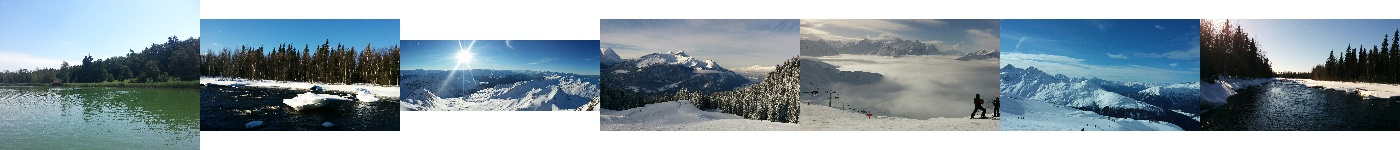
\includegraphics[width=1.0\columnwidth]{../figures/top7_suitable.jpg}
\caption{Top 7 suitable images in descending score order (Michael dataset)\label{fig:selection_top7}}
\end{figure}

Figure \ref{fig:selection_out1} shows 21 sample images from the Michael dataset.
These images, as mentioned before, can include undesirable objects such as text,
street signs, or store items.
As mentioned in section \ref{sec:method_cropping}, a SVM is trained using
features representing object classes.
When classifying the given images using this SVM, the resulting selection of
wallpaper candidates are shown in figure \ref{fig:selection_out2}.

\begin{figure}
\centering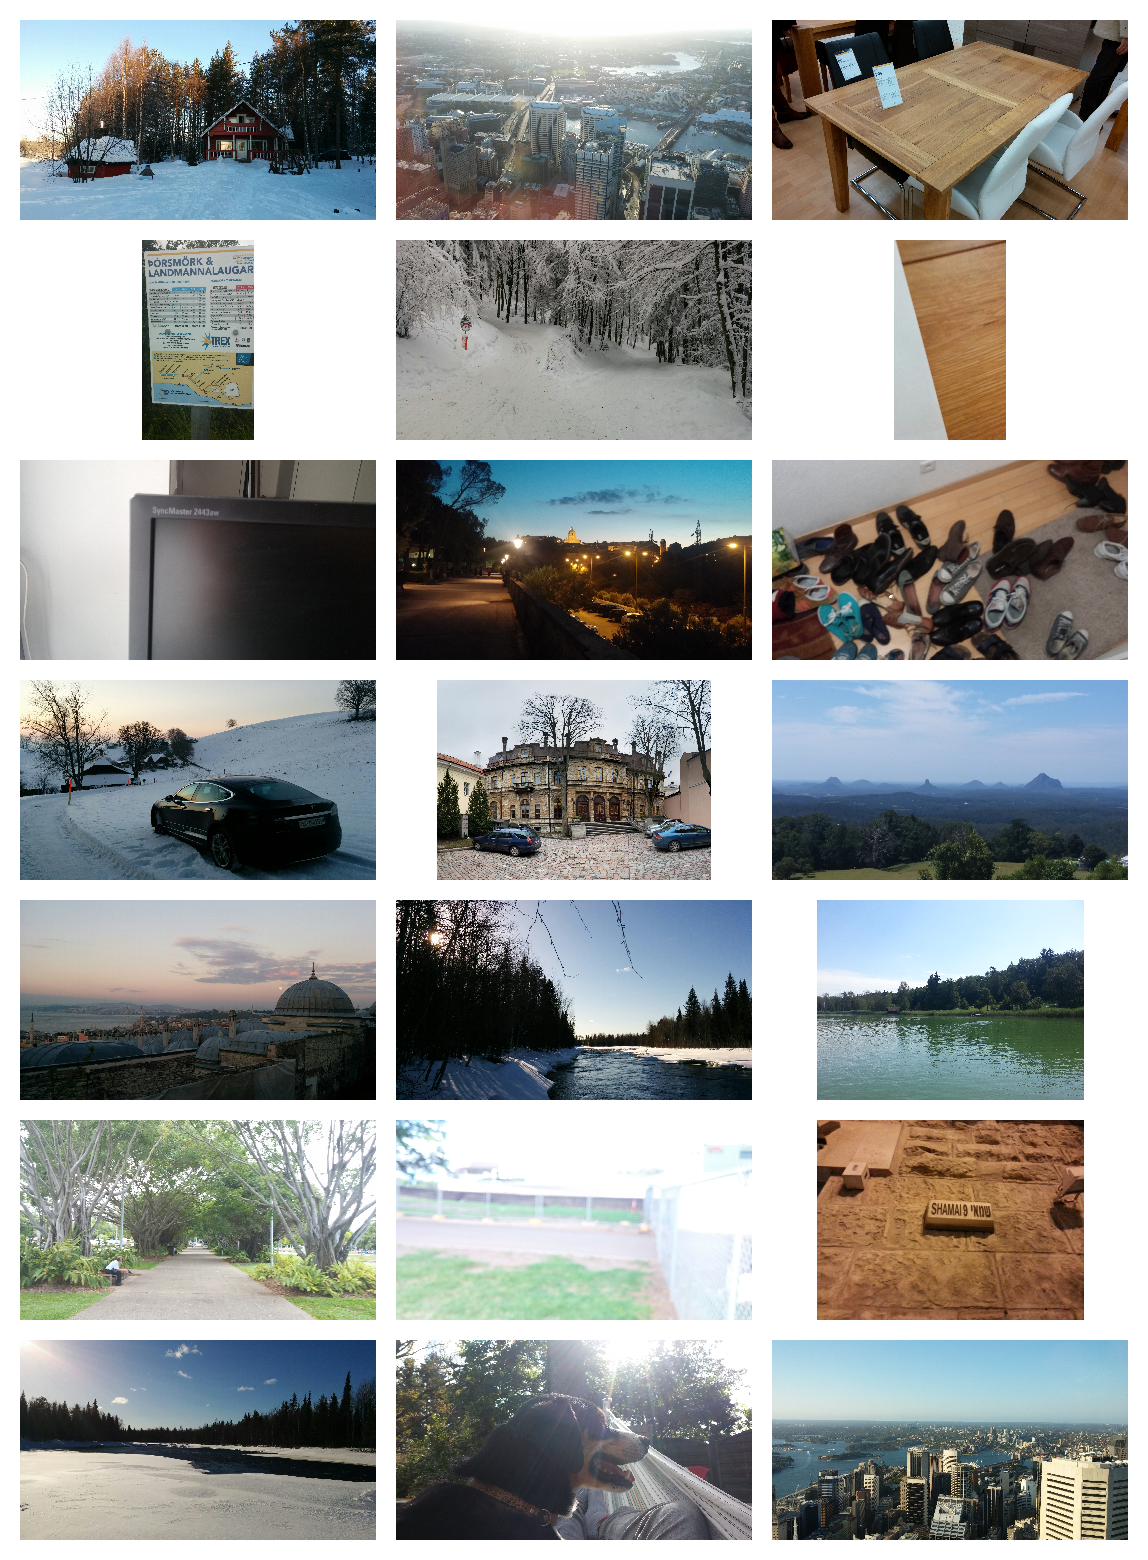
\includegraphics[width=0.9\columnwidth]{../figures/grid7x3_out1.png}
\caption{21 sample images from Michael dataset.\label{fig:selection_out1}}
\end{figure}

It can be seen qualitatively that images with undesirable objects have been
discarded, such as the image of furniture, a poster, or the model number
of electronic equipment.
Though in general photos with obviously undesirable objects are discarded, photos of city skylines or prominent single foreground objects for example are not usually classified as being appropriate.
This is due to disagreements between annotators.
A larger number of annotations per image may help in this case.

\begin{figure}
\centering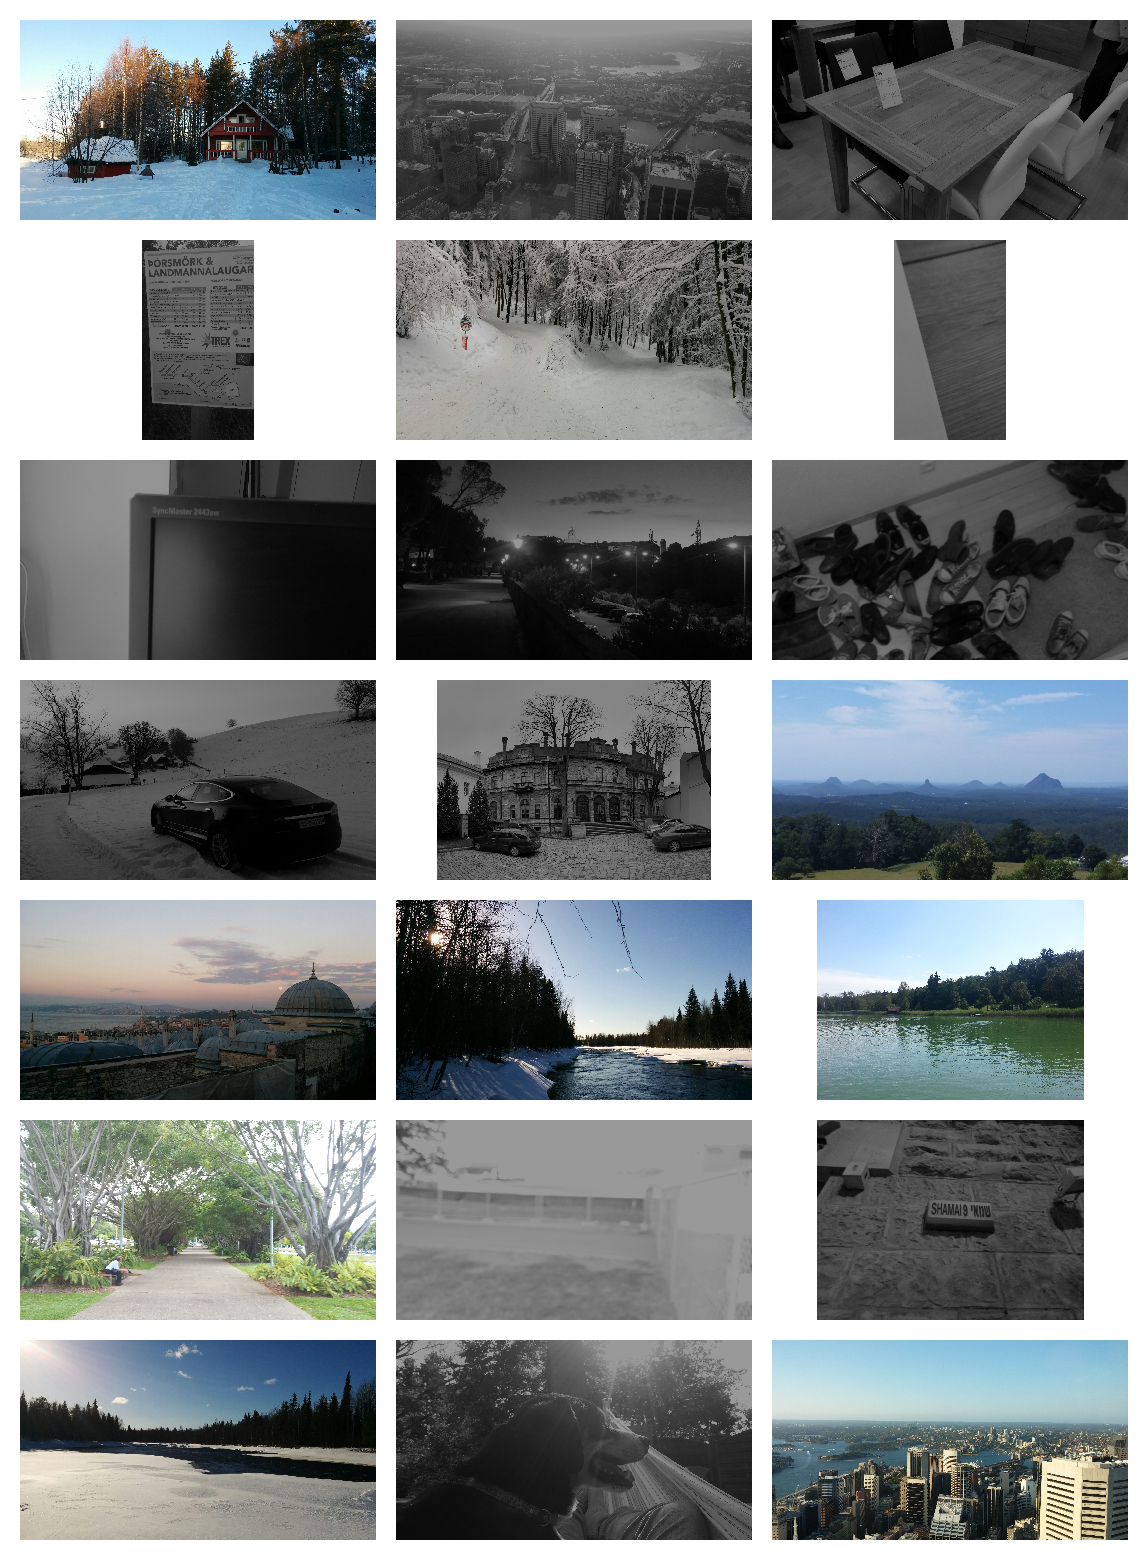
\includegraphics[width=0.9\columnwidth]{../figures/grid7x3_out2.png}
\caption{21 sample images from Michael dataset with images not selected dimmed
	and in grayscale.\label{fig:selection_out2}}
\end{figure}

When evaluating scores for all images in the Michael dataset, it can be seen in
figure \ref{fig:selection_top7} that images of distant natural landscapes attain
high scores.
Unlike scenes such as dark indoors and cityscapes, natural landscapes tend to be
classified as suitable by more annotators.

It should be noted that a single user's preference could be greatly different
from most other users where the purpose and intent of having a photo wallpaper
may differ.
For example, user A may desire to have dark and slightly artistic photos mainly
biasing towards indoor club scenes and long exposure shots at night.
User B might be a big fan of album art or concert photos, desiring objects or
scenes that we tend to assume to be undesirable.
It was actually the case in this study that using greatly conflicting
annotations caused issues in classification, where an annotator heavily favoured
dark scenes with low detail or discernible objects.

Further work could be done to perform a weighted average of multiple classifiers
depending on wallpaper preferences.

\newpage
\section{Cropping\label{sec:qualitative_cropping}}

As we have seen in section \ref{sec:quant_cropping}, the cropping algorithm performs well compared to previous works.
We now assess how well the algorithm works in practise with the image dataset provided by \cite{fang2014automatic}.

In the following figures, four images are shown per input image: the original
image, a saliency map, a gradient map, and the final cropped image.
It should be noted that brigher regions in a saliency map represent more
visually distinct regions, and brighter regions in a gradient map represent
regions with large changes in colour.

It is hoped that the saliency map emphasizes prominent objects well enough for
irrelevant or less important details to be left out of the final crop, and the
gradient map exhibit high values for boundaries and detailed foreground objects.
For the cases where this is true, it can be seen that the algorithm works very
well.

In figure \ref{fig:cropped_refocus} in particular, it can be seen that the most
prominent object is retargeted well.
This tends to result in better composed final images.
Some of the crops even exhibit some considerations of boundary simplicity.
Figure \ref{fig:cropped_simplicity} shows this effect better.
The classifier favours having lower gradient values on crop borders, leading to
crops which do not tend to intersect objects.
It should be noted that since the input gradient map is intentionally not
normalised, weaker boundaries can be included in crop boundaries.
As opposed to \cite{fang2014automatic}, the weighting of boundary simplicity is
not done using a fixed variable but by relying on the training of the SVM.

\begin{figure}
\centering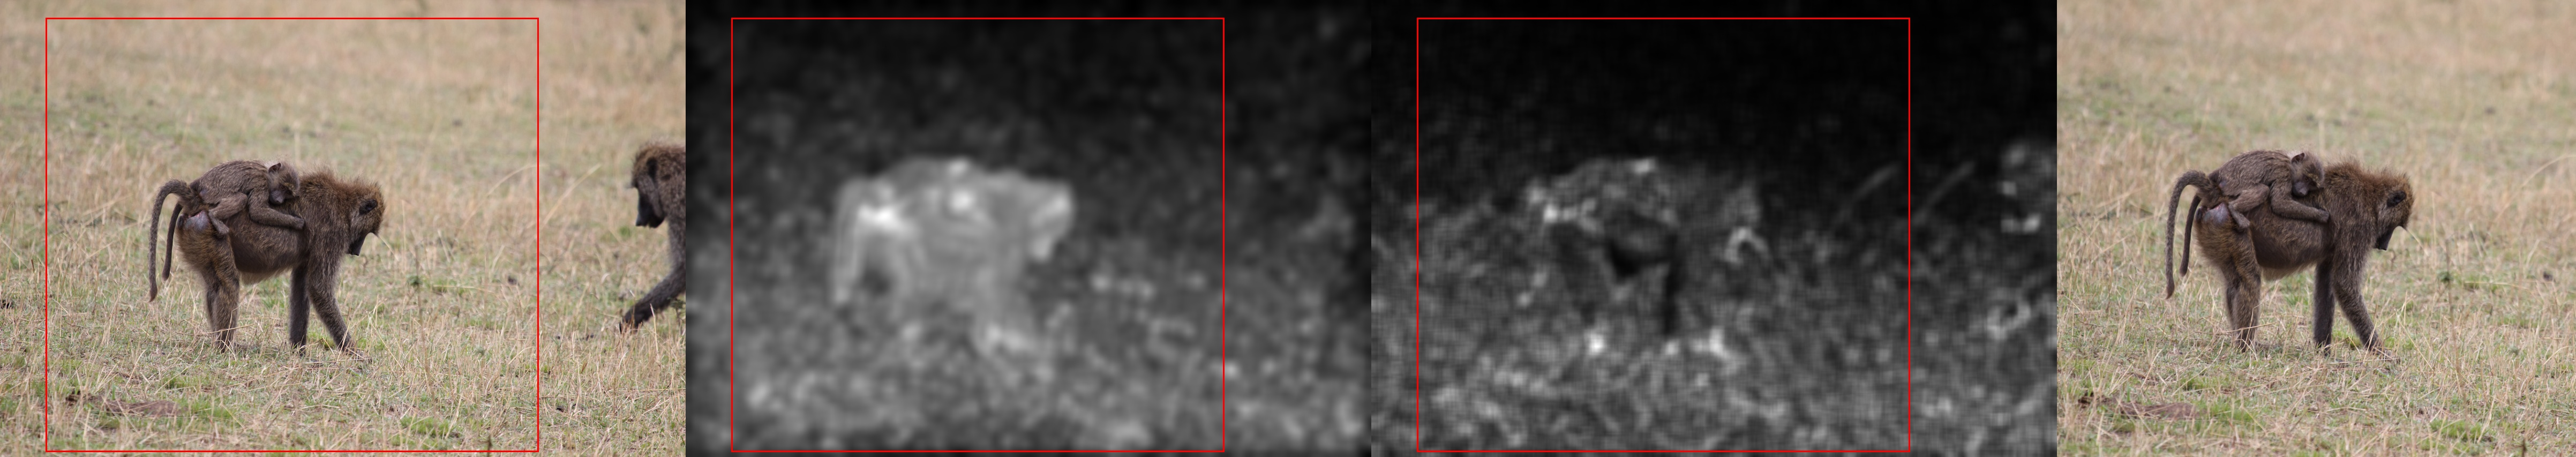
\includegraphics[width=0.9\columnwidth]{../figures/Chen_crops/isolate/IMG_0350.jpg}
\vskip3pt
\centering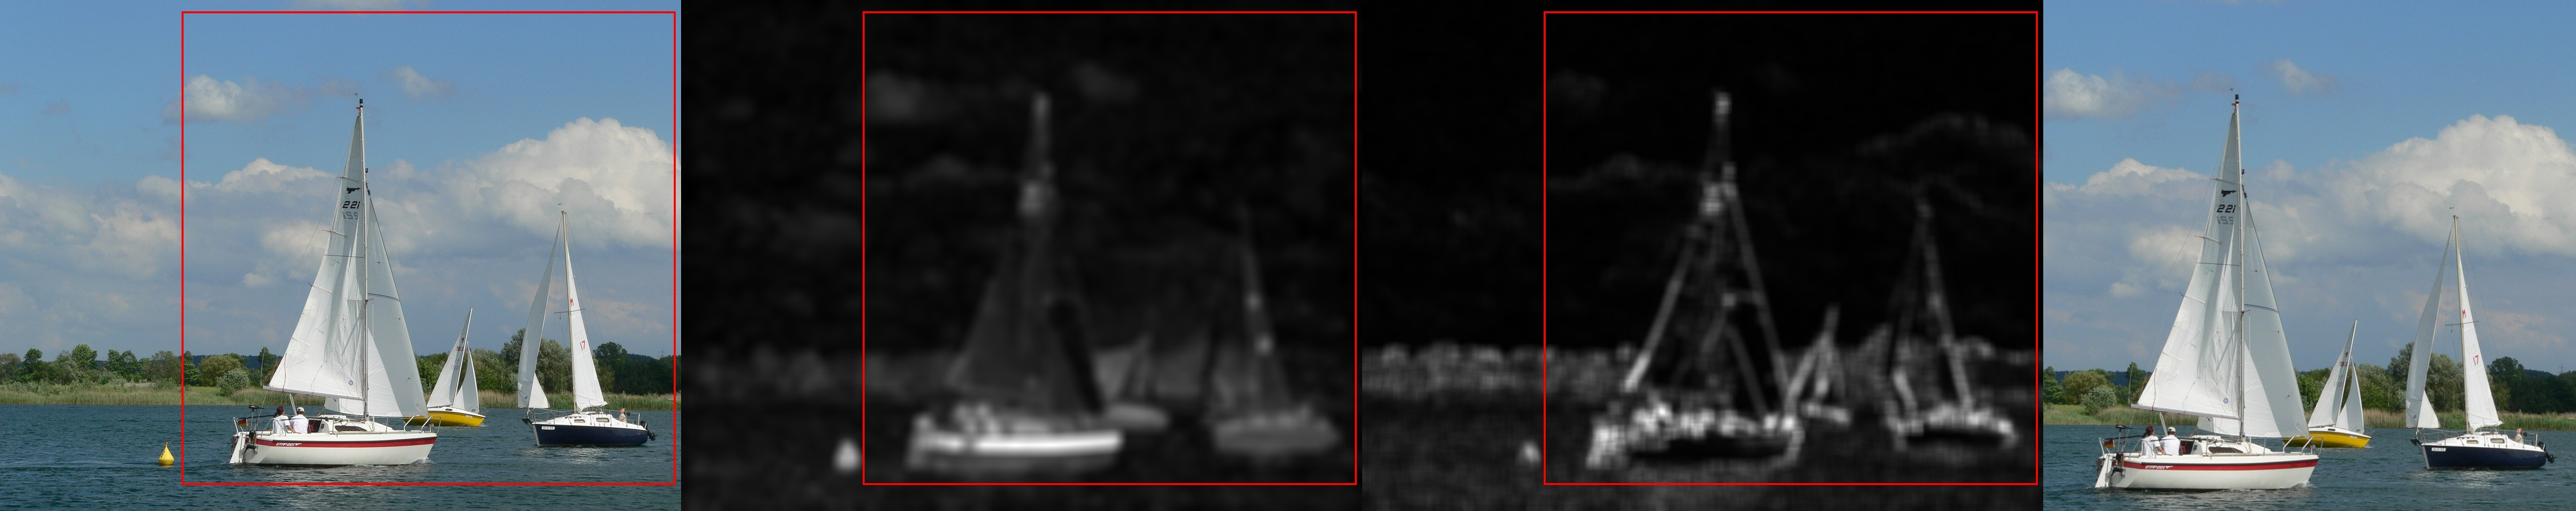
\includegraphics[width=0.9\columnwidth]{../figures/Chen_crops/refocus/146931510_Large.jpg}
\vskip3pt
\centering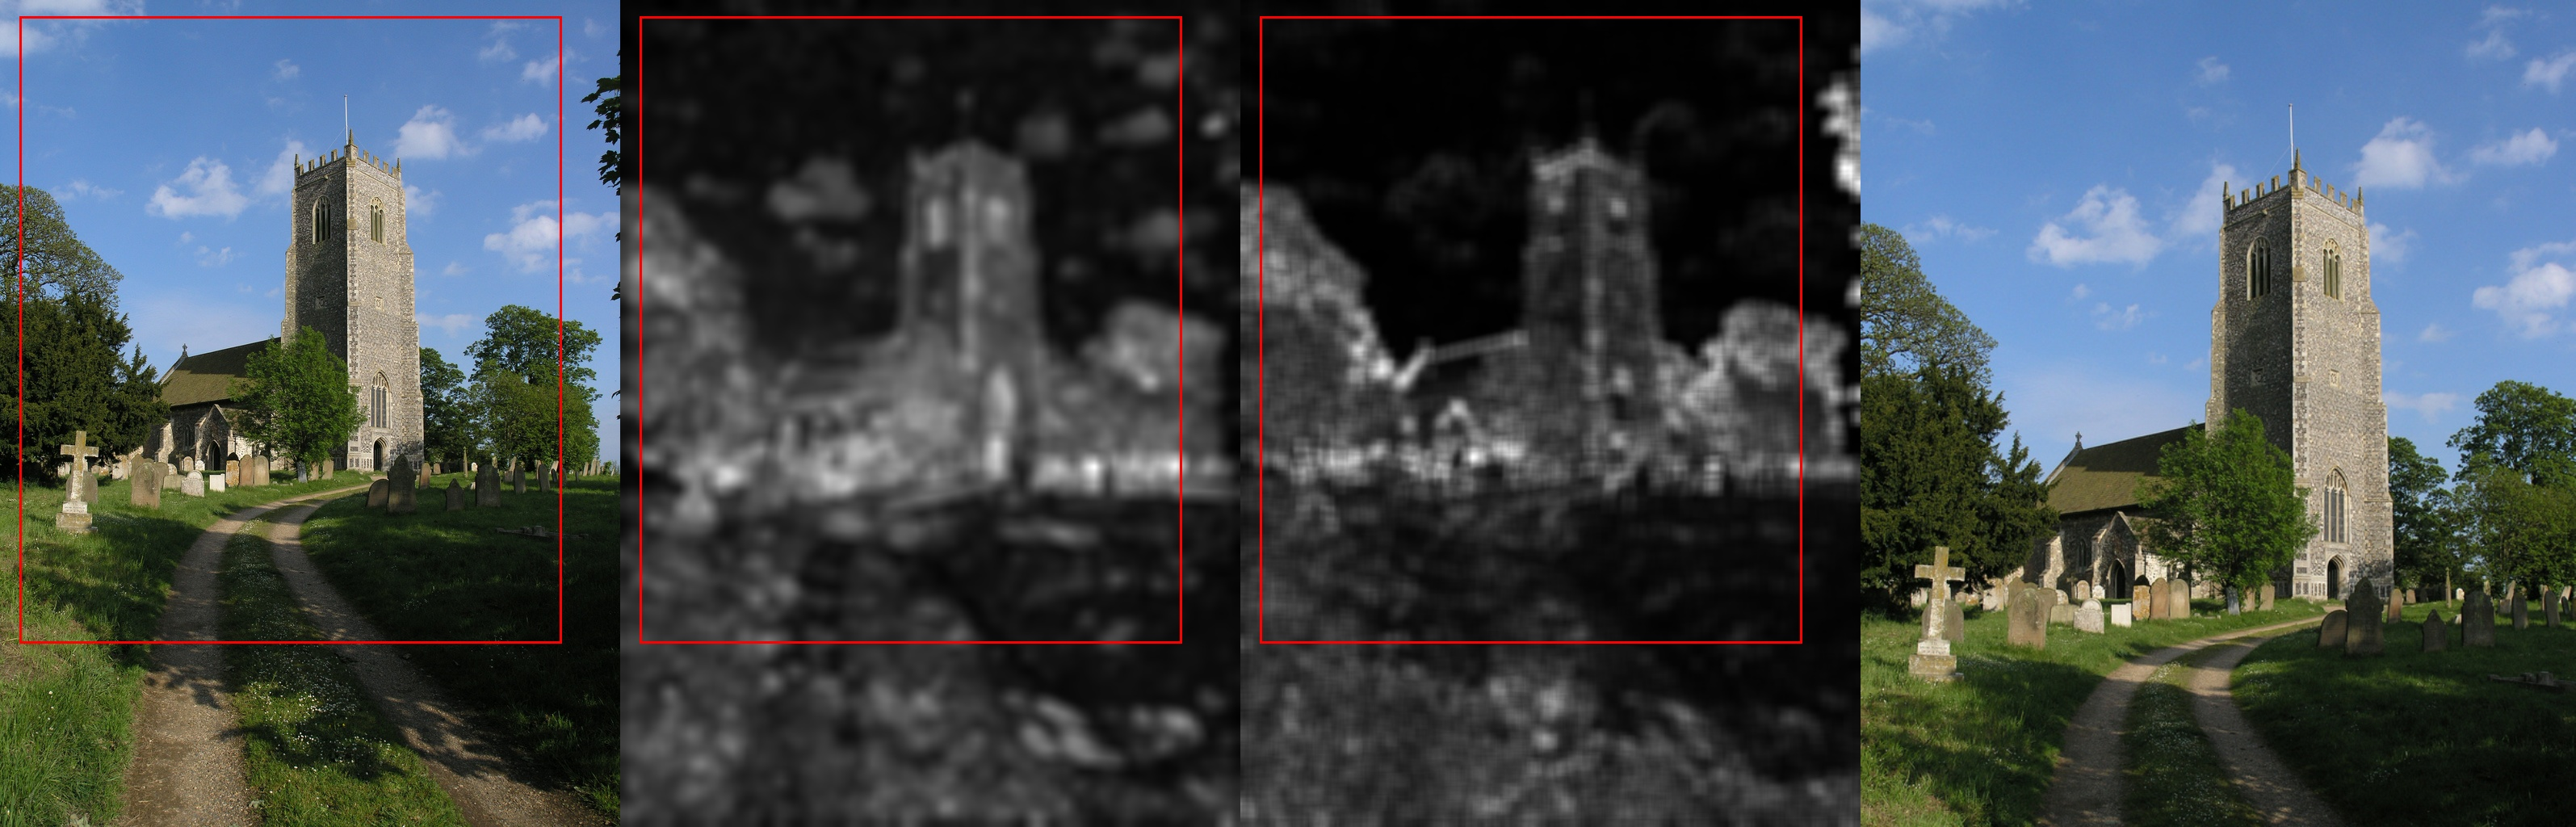
\includegraphics[width=0.9\columnwidth]{../figures/Chen_crops/refocus/1845766133_Large.jpg}
\vskip3pt
\centering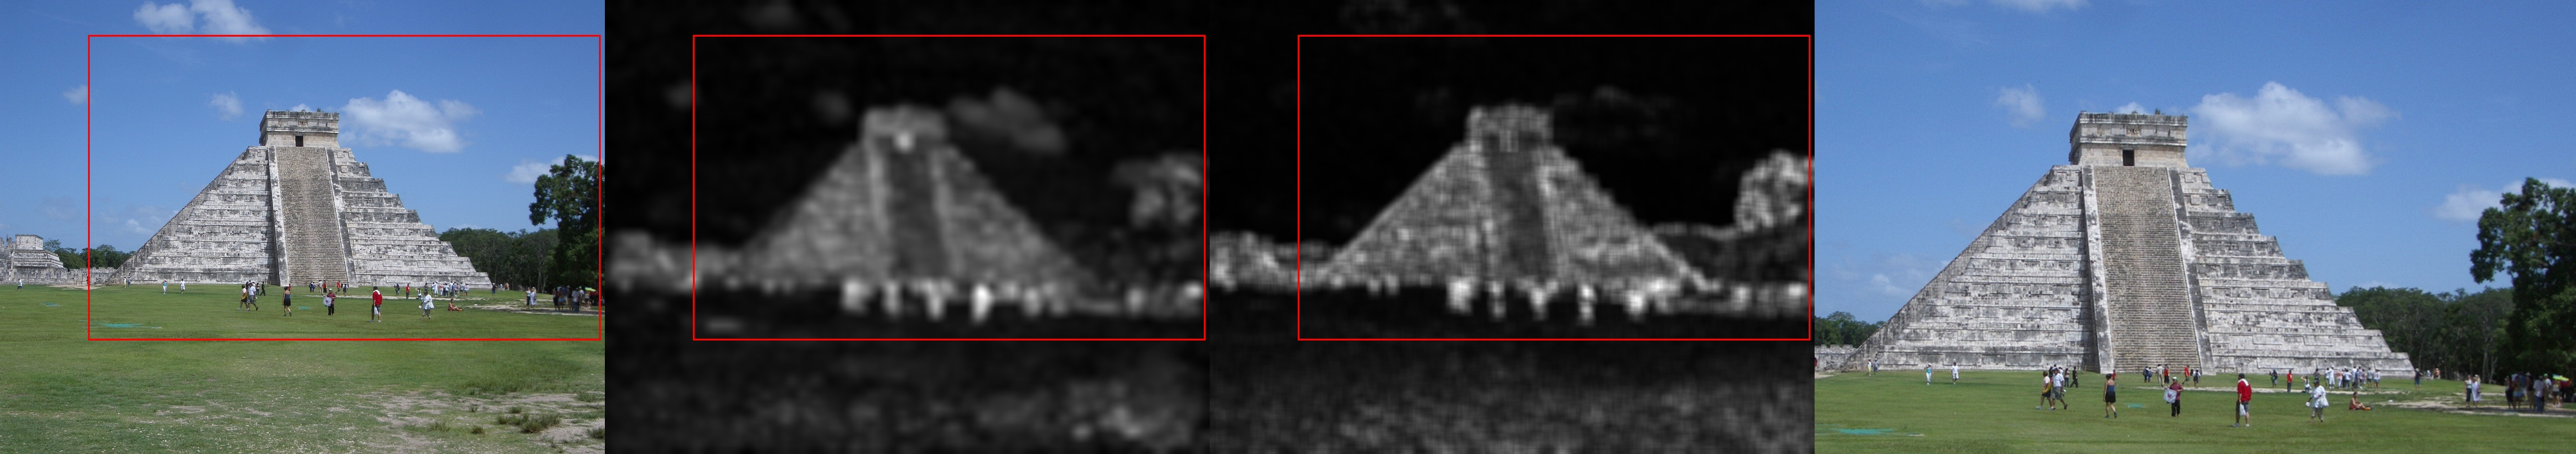
\includegraphics[width=0.9\columnwidth]{../figures/Chen_crops/refocus/236441280_Large.jpg}
\vskip3pt
\centering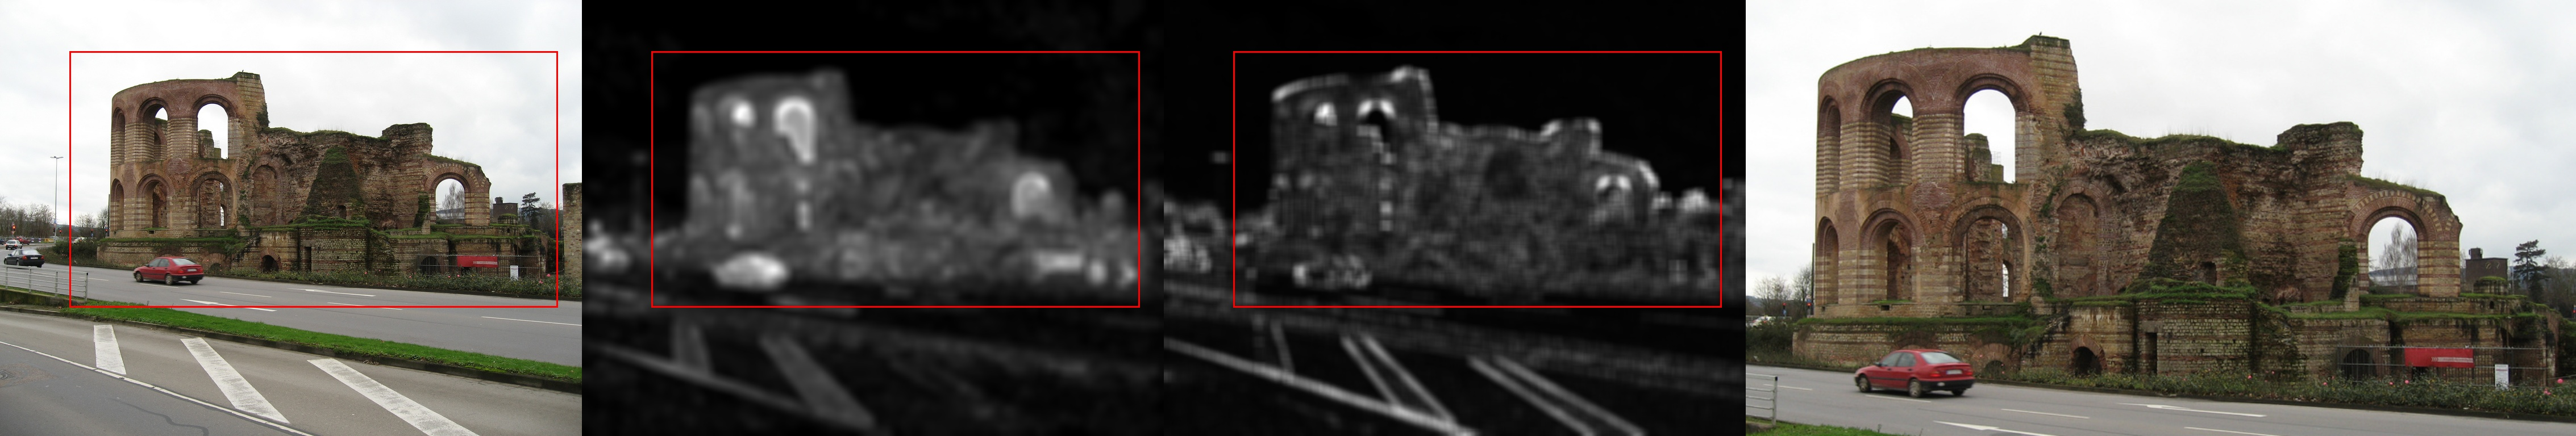
\includegraphics[width=0.9\columnwidth]{../figures/Chen_crops/refocus/406813066_Large.jpg}
\vskip3pt
\centering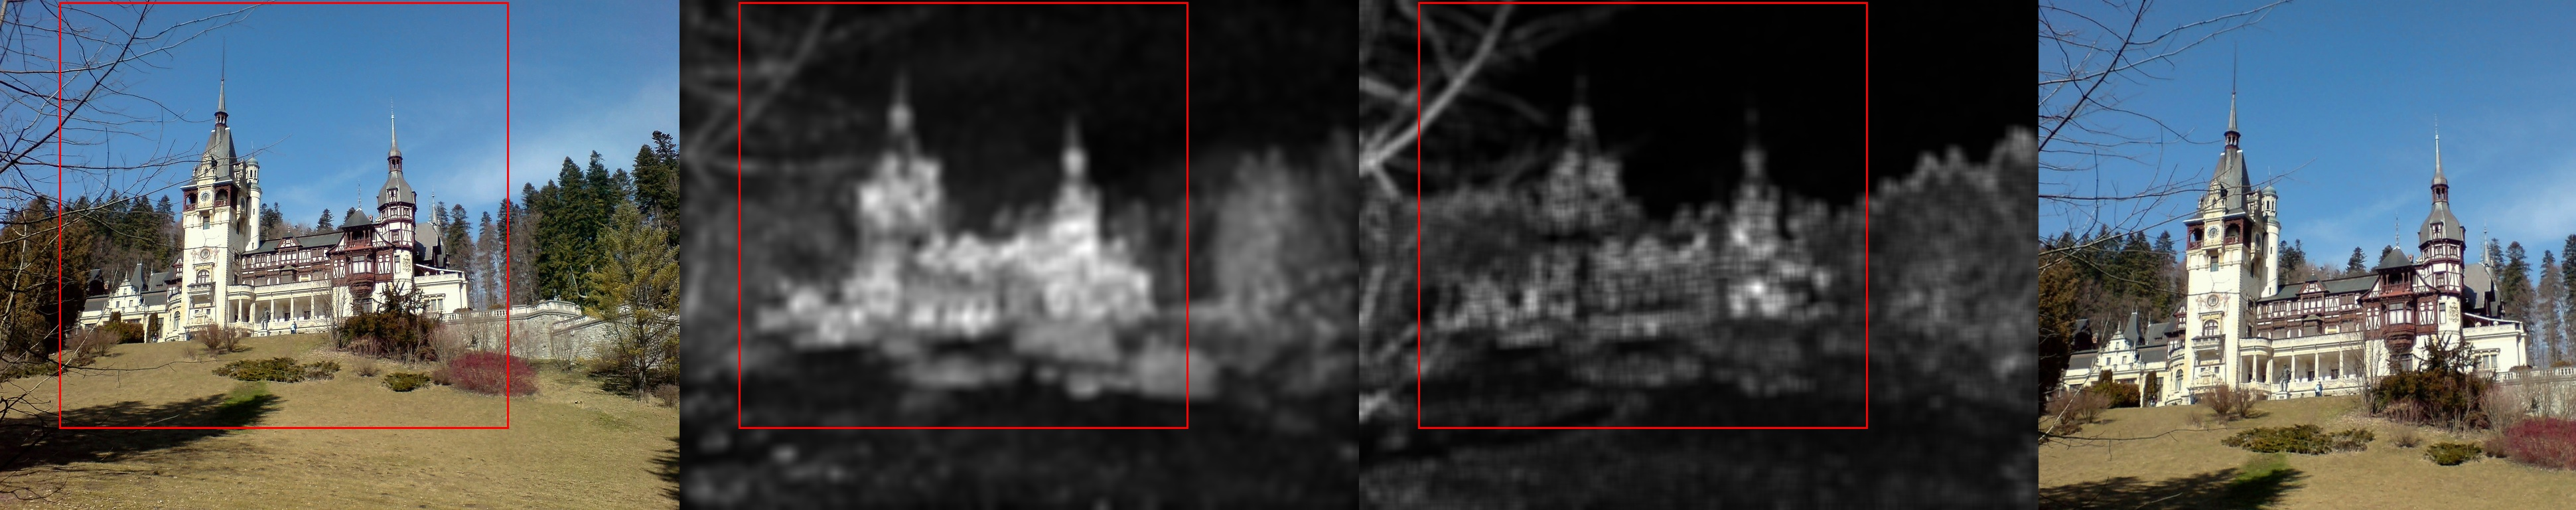
\includegraphics[width=0.9\columnwidth]{../figures/Chen_crops/refocus/420319741_Large.jpg}
\vskip3pt
\small{(From left to right: original image, saliency map, gradient map, final cropped image)}
\caption{Crops with main objects isolated and centered.\label{fig:cropped_refocus}}
\end{figure}

\begin{figure}
\centering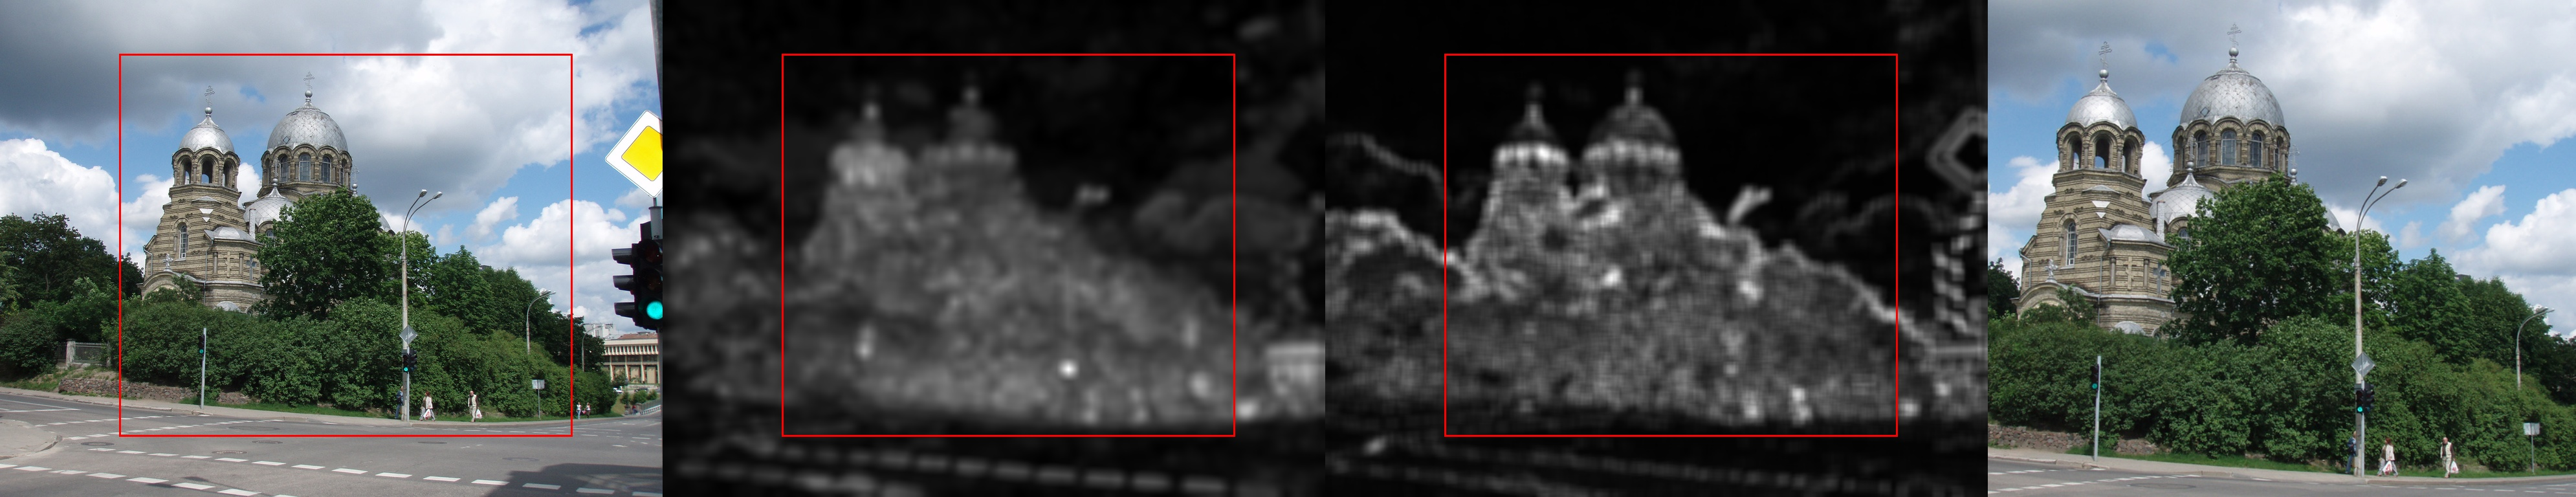
\includegraphics[width=0.9\columnwidth]{../figures/Chen_crops/simple_boundary/1022974255_Large.jpg}
\vskip3pt
\centering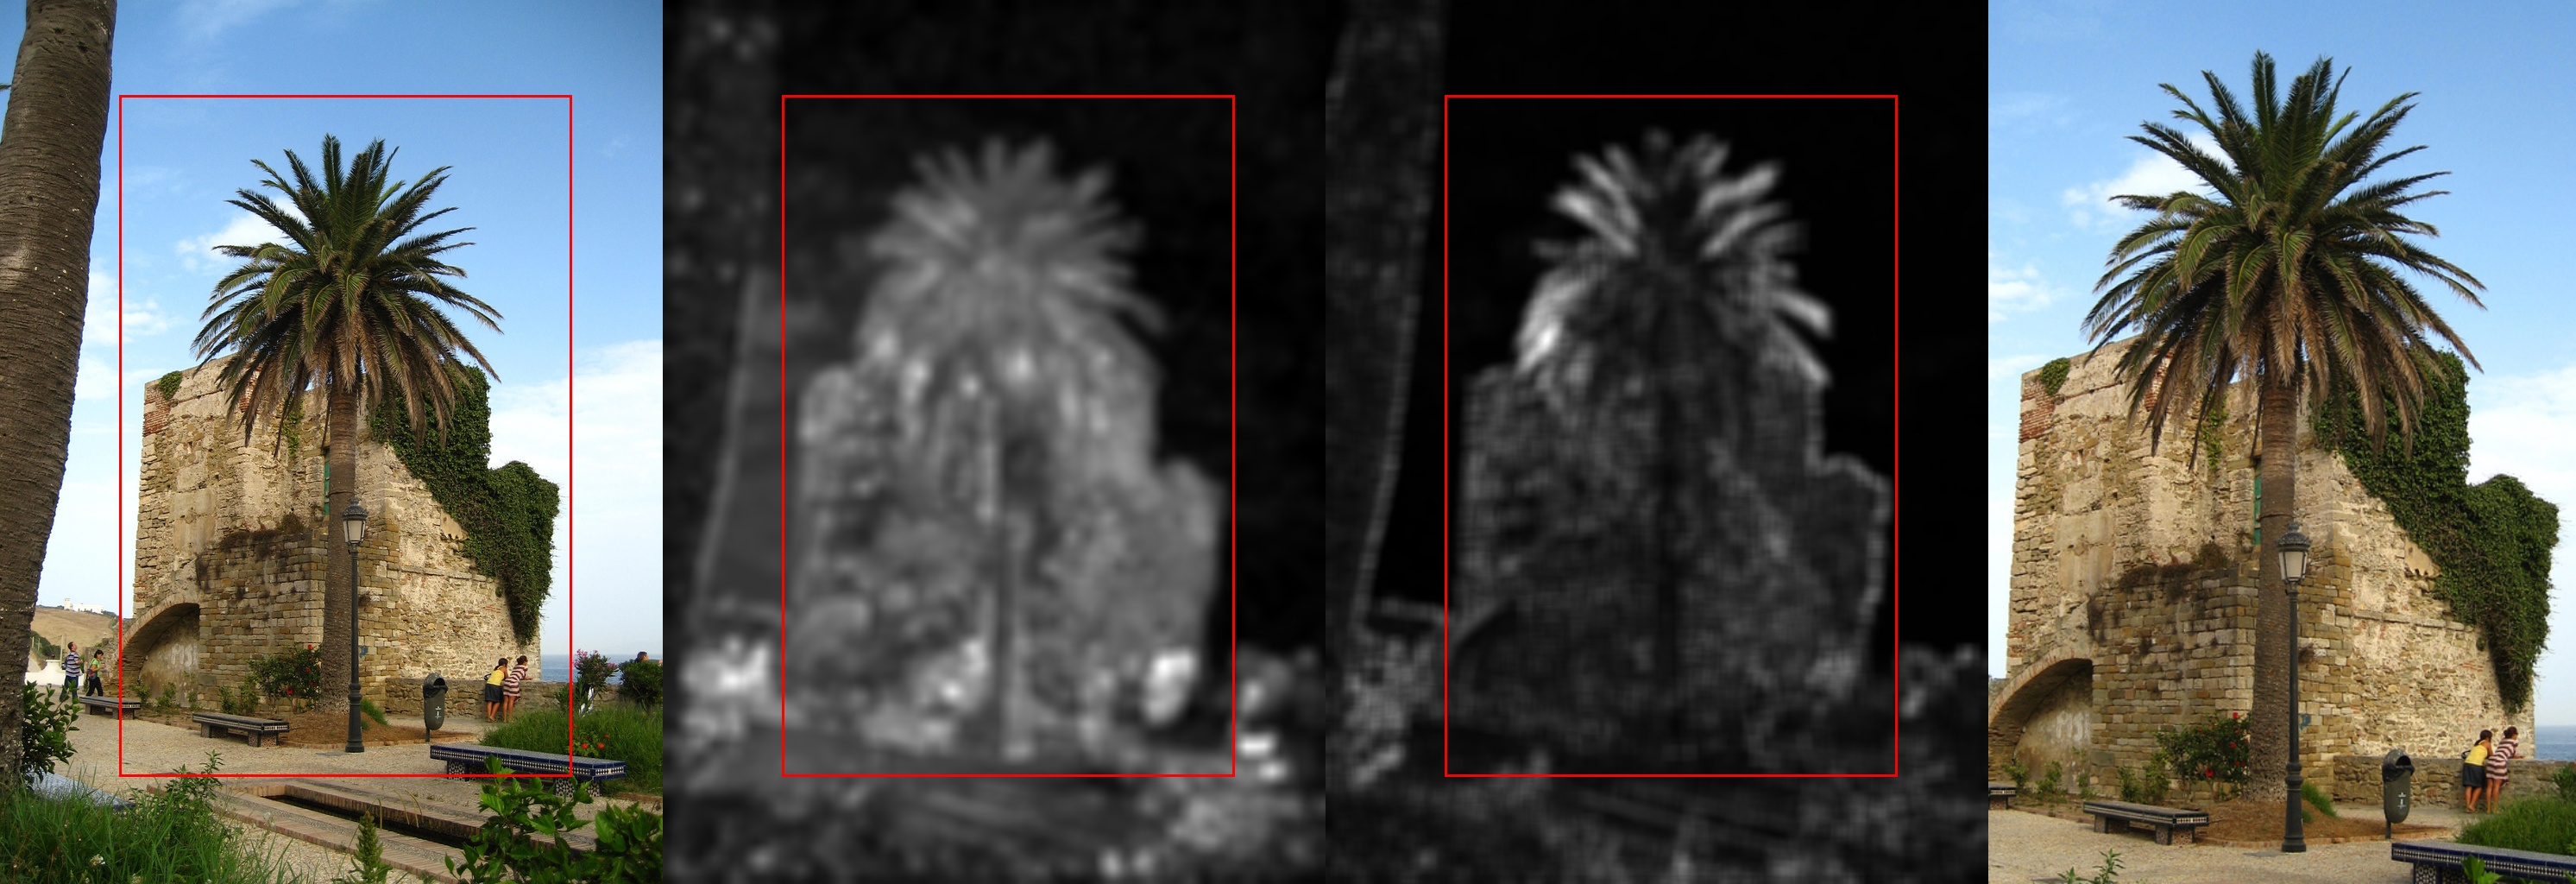
\includegraphics[width=0.9\columnwidth]{../figures/Chen_crops/simple_boundary/1192872104_Large.jpg}
\vskip3pt
\centering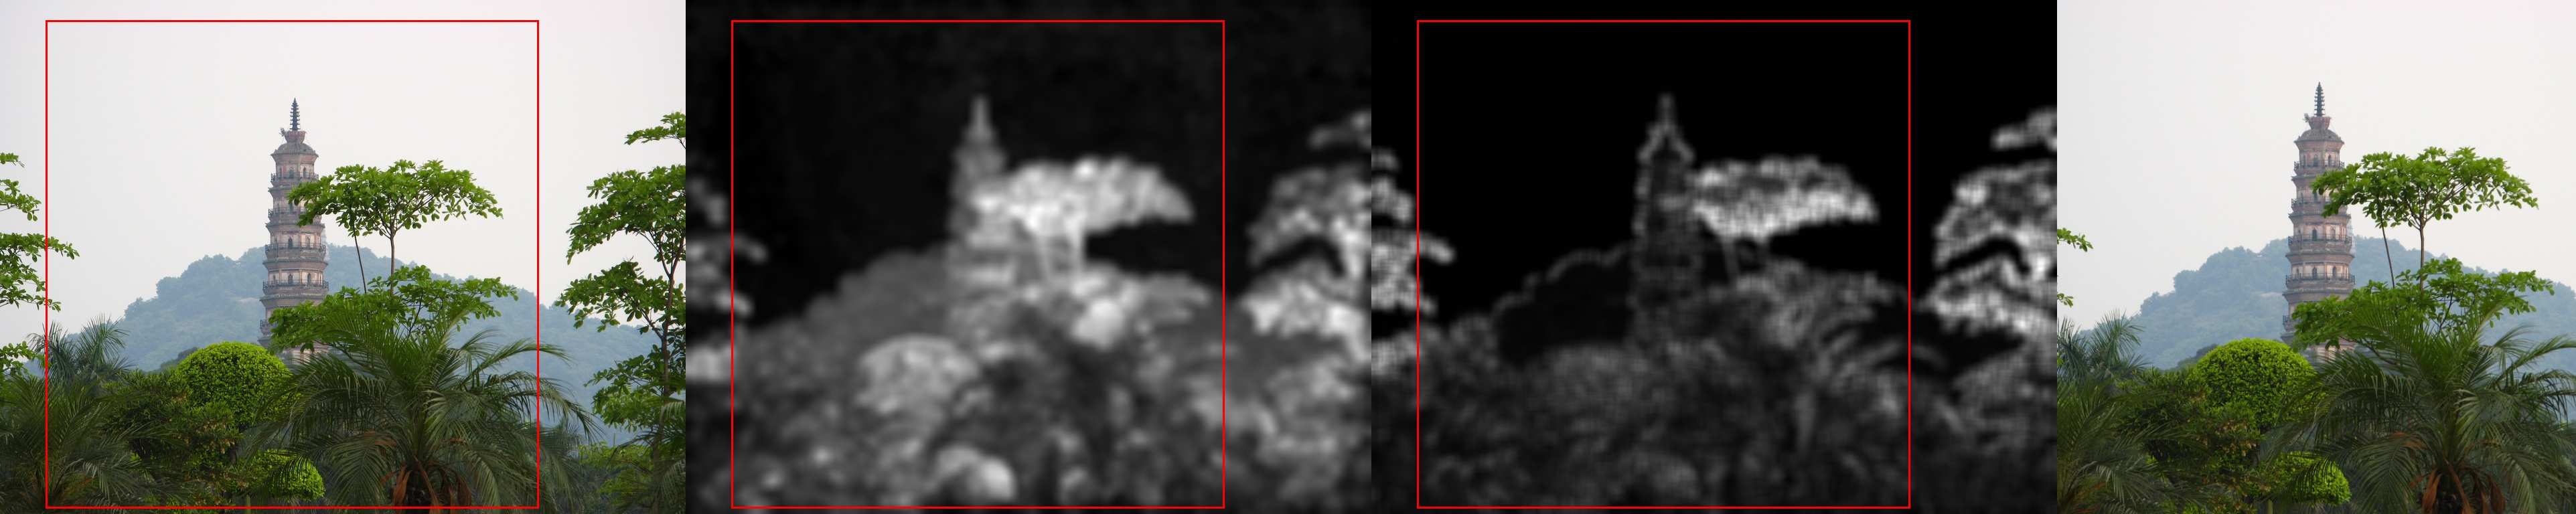
\includegraphics[width=0.9\columnwidth]{../figures/Chen_crops/simple_boundary/504325680_Large.jpg}
\vskip3pt
\centering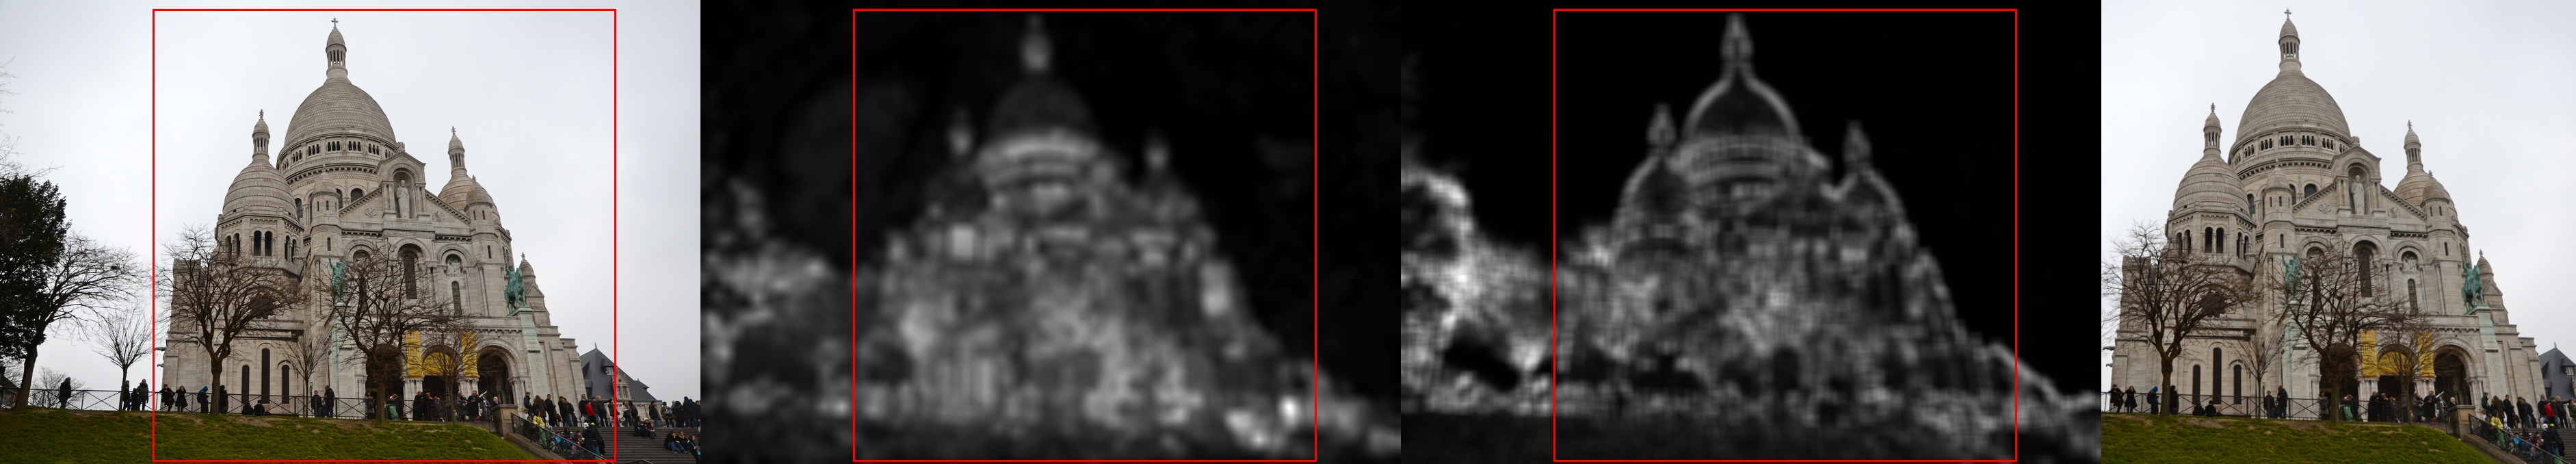
\includegraphics[width=0.9\columnwidth]{../figures/Chen_crops/simple_boundary/6853433974_Large.jpg}
\vskip3pt
\small{(From left to right: original image, saliency map, gradient map, final cropped image)}
\caption{Crops with good boundary simplicity.\label{fig:cropped_simplicity}}
\end{figure}

The automatic cropper does have its pitfalls however.
The most common error occurs when the final crop cuts through distinct
foreground objects.
This is shown well in figure \ref{fig:cropped_cutobject}.
It can be seen especially well for the case of the first image that the fault
may lie in the saliency map implementation used.
Other background colours and patterns are deemed more salient at times making
it more challenging for the algorithm to retain relevant but "not salient"
regions.

\begin{figure}
\centering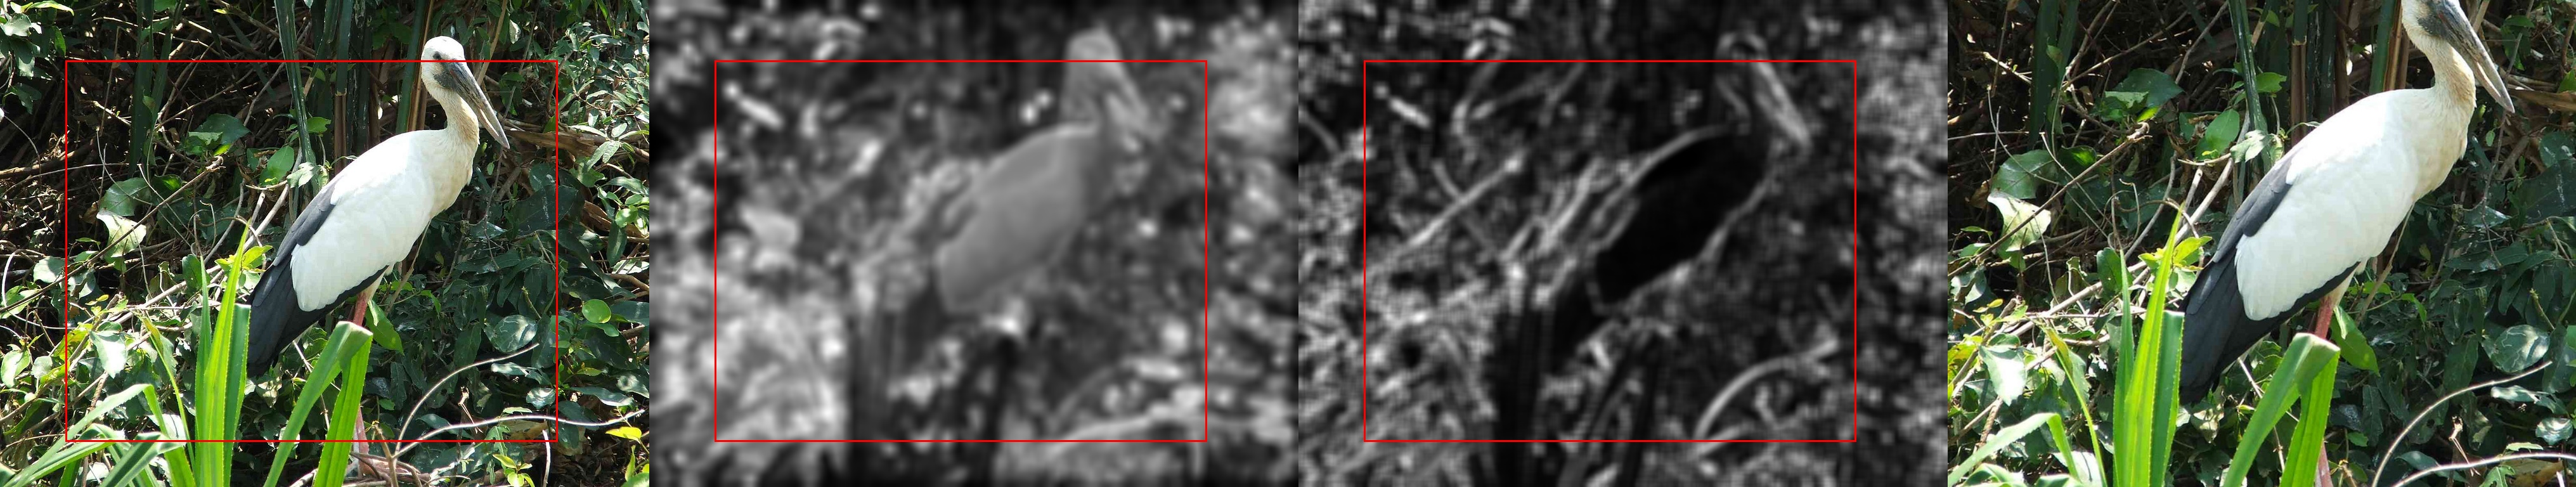
\includegraphics[width=0.9\columnwidth]{../figures/Chen_crops/cut_object/118697470_Large.jpg}
\vskip3pt
\centering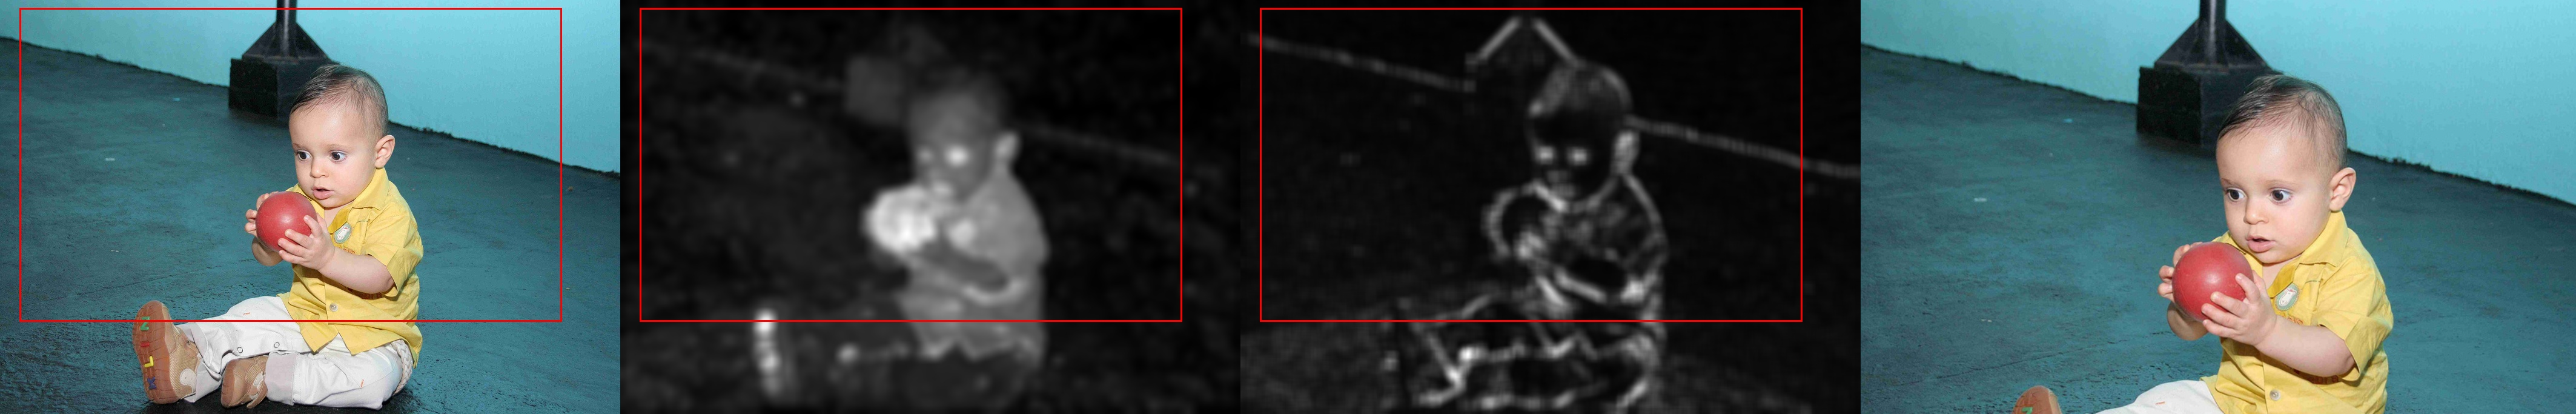
\includegraphics[width=0.9\columnwidth]{../figures/Chen_crops/cut_object/1347846010_Large.jpg}
\vskip3pt
\centering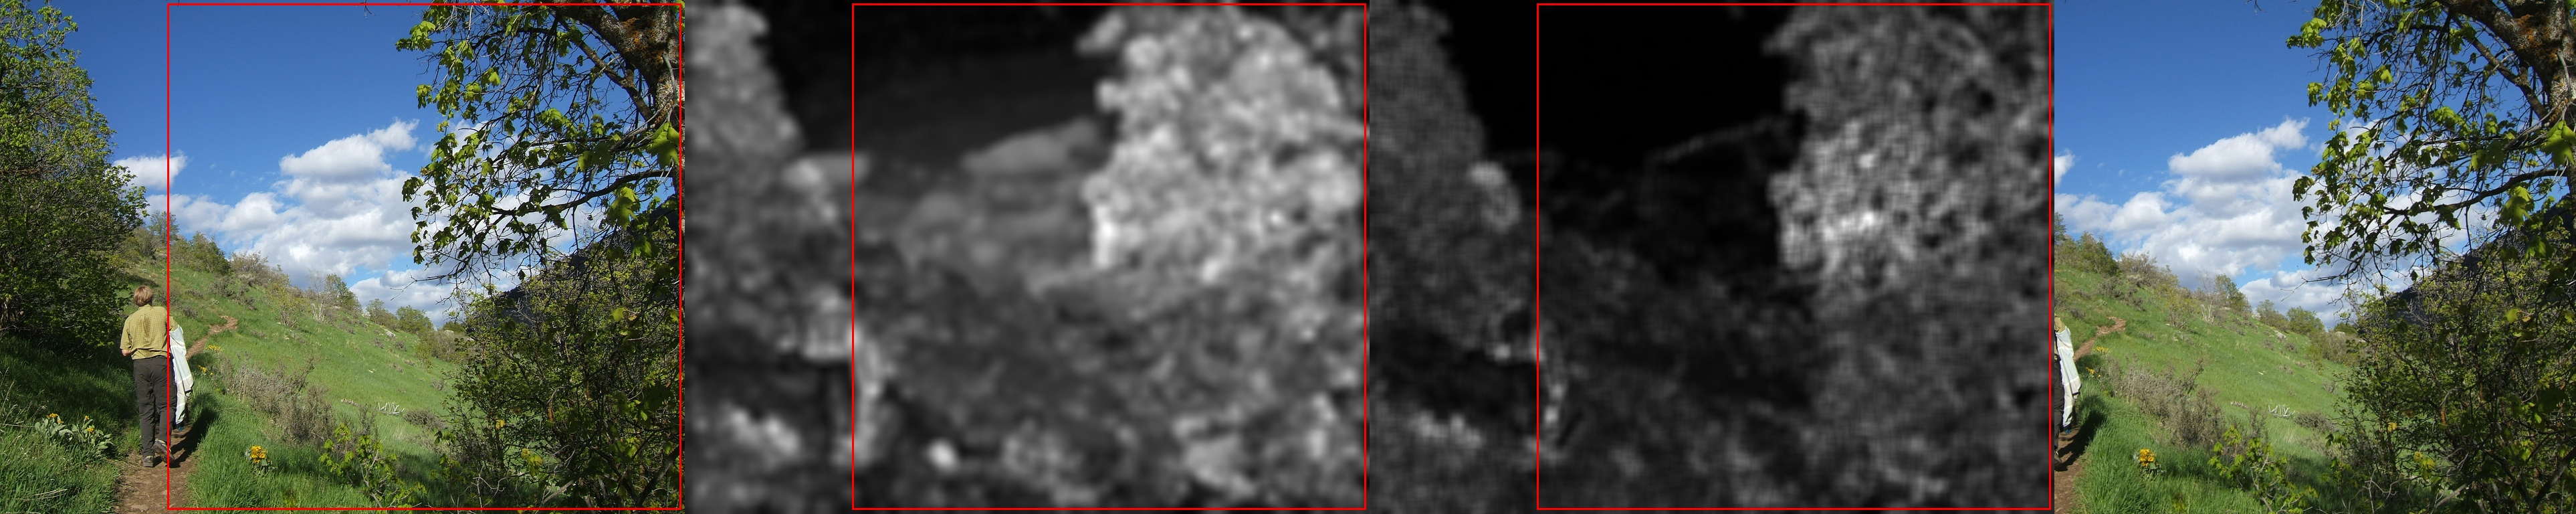
\includegraphics[width=0.9\columnwidth]{../figures/Chen_crops/cut_object/490466578_Large.jpg}
\vskip3pt
\centering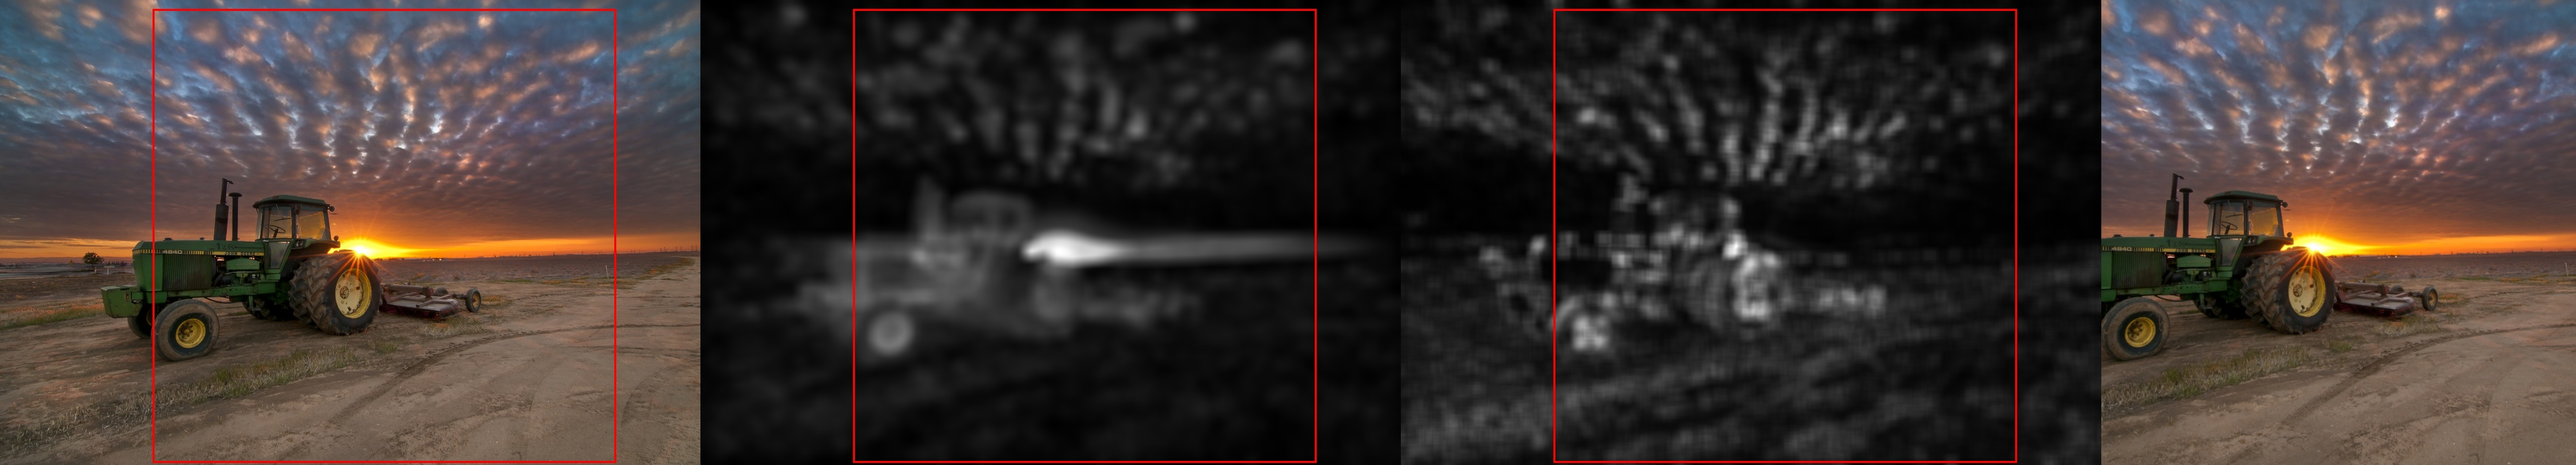
\includegraphics[width=0.9\columnwidth]{../figures/Chen_crops/cut_object/6853040778_Large.jpg}
\vskip3pt
\small{(From left to right: original image, saliency map, gradient map, final cropped image)}
\caption{Unideal crops which cut through objects.\label{fig:cropped_cutobject}}
\end{figure}

Another example where the saliency map implementation may cause issues is when
reflections occur in an input image.
Figure \ref{fig:cropped_reflection} shows an example with a flock of flamingoes
and their reflection.
Both the flock and their reflection is considered salient and thus the final
crop is not composed as well as the initial image.
This could be a cause for confusion for human croppers as well however,
especially when a reflection could be considered artistic and thus should be
well focused.

\begin{figure}
\centering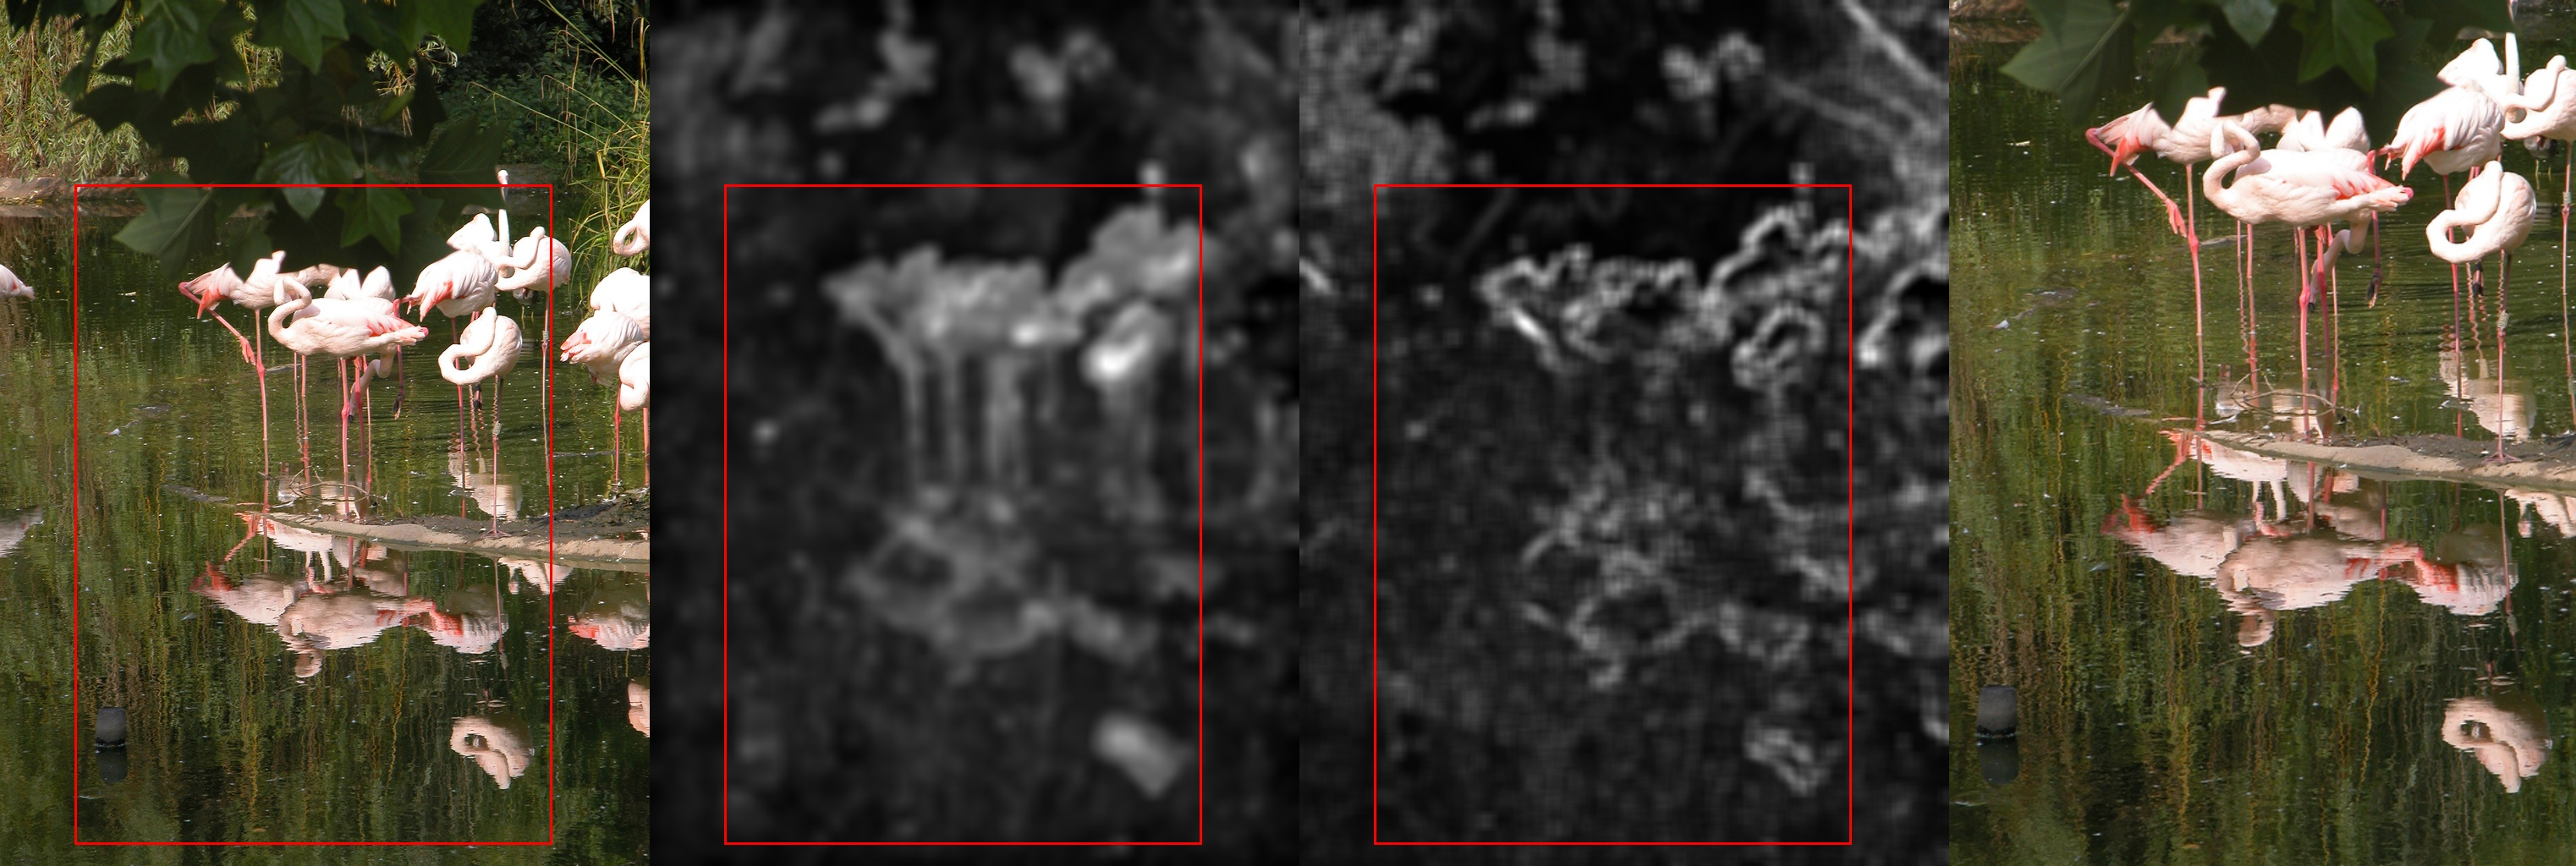
\includegraphics[width=0.9\columnwidth]{../figures/Chen_crops/reflections/46152273_Large.jpg}
\vskip3pt
\small{(From left to right: original image, saliency map, gradient map, final cropped image)}
\caption{Unideal crop due to reflections.\label{fig:cropped_reflection}}
\end{figure}

Overall, the automatic cropping algorithm works very well.
Any mistakes could be improved in the future with better saliency map
implementations.



%% ----------------------------------------------------------------------------
% BIWI SA/MA thesis template
%
% Created 09/29/2006 by Andreas Ess
% Extended 13/02/2009 by Jan Lesniak - jlesniak@vision.ee.ethz.ch
%% ----------------------------------------------------------------------------
\newpage
\chapter{Quantitative Analysis\label{sec:quantitative}}

\section{Selection}

4 volunteers were asked to annotate the wallpaper datasets.
For the Michael dataset, there is a correlation coefficient ($R$) of 0.49 in
annotations, while $R=0.28$ for the Wookie dataset.
It could already be seen that the Michael dataset is perhaps of higher quality
in terms of variety of objects imaged and lower repetitions.

When training a model on the Michael dataset and evaluating the model on the
Wookie dataset, there are 5 incorrect predictions for 135 images where
annotations agree.
This is an error rate of $3.7\%$, much lower than the opposite where training is
performed on the Wookie dataset and evaluation done on the Michael dataset.
In this case, there are 42 incorrect predictions for 141 images where
annotations agree.
This is a $29.8\%$ error, confirming that the quality of the Wookie dataset
could be improved.

Furthermore, we evaluate the performance of the classifier when training on
one's own annotations vs training on all available annotations.
While this error fluctuates for each annotator, the average error is $59.2\%$
for the case where training is performed using all available annotations.
This is a much higher error compared the case when training is only done using
an annotator’s own annotations ($29.2\%$ error).
An interesting study would be to see if combining annotations with high
correlation helps to improve the performance of the personalised classifier
of a user.

Another analysis done is the assessment of the Precision-Recall curve of the
classifiers (figure \ref{fig:PR}).
This is for the case when training on all annotations for either datasets and
evaluating on the other dataset.
For both cases, the trained models exhibit higher precision than the case where a random classifier is used.
The decision function of a random classifier returns a uniformly distributed random number in the range of expected values.
It can therefore be concluded that the classifiers serve their purposes.
In the case of the model trained on the Wookie set however, the base precision of $0.4$ is quite high, indicating that the annotations may not be well balanced.

\begin{figure}
\centering
\begin{subfigure}{0.79\columnwidth}
  \centering
  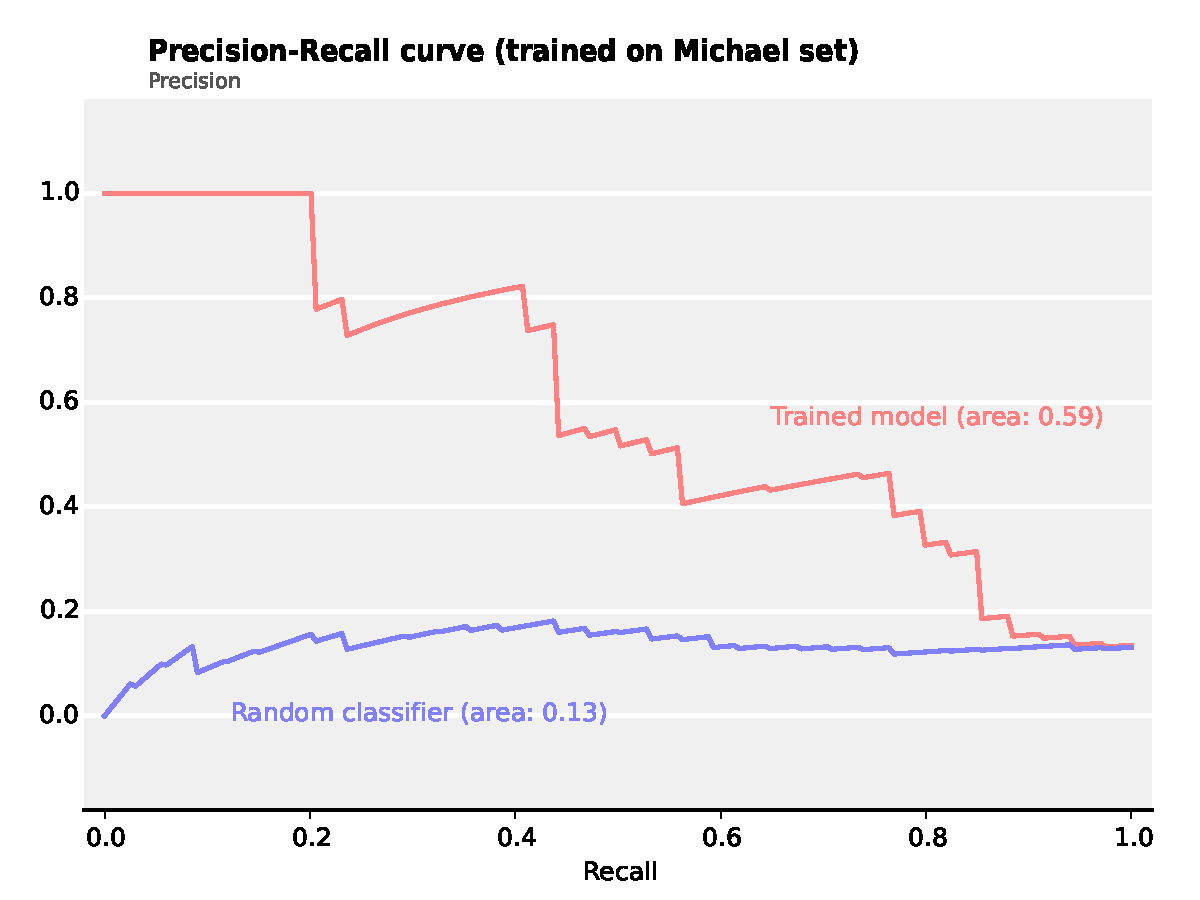
\includegraphics[width=0.99\columnwidth]{../figures/PRcurve_michael_wookie.pdf}
  \caption{Classifier trained on Michael set, evaluated on Wookie set.}
\end{subfigure}
\vskip8mm
\begin{subfigure}{0.79\columnwidth}
  \centering
  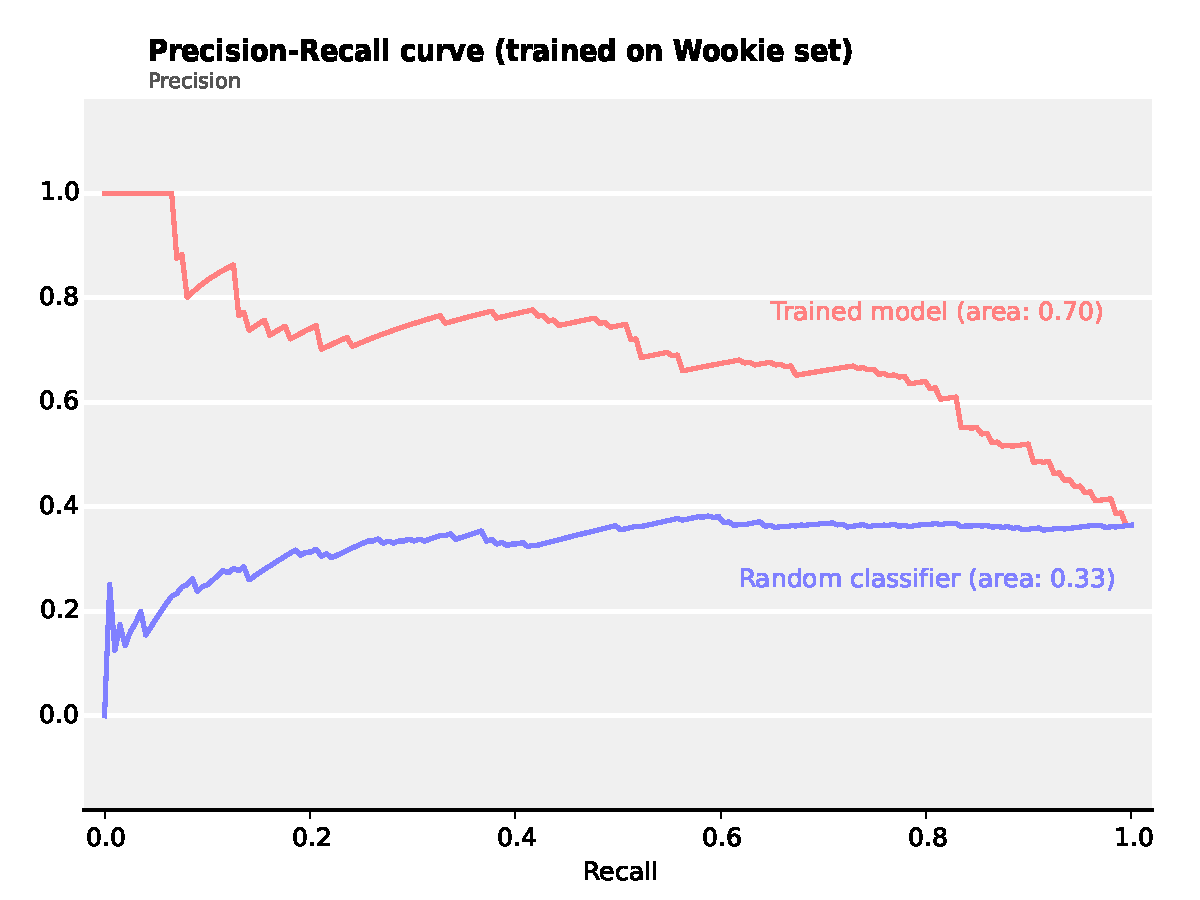
\includegraphics[width=0.99\columnwidth]{../figures/PRcurve_wookie_michael.pdf}
  \caption{Classifier trained on Wookie set, evaluated on Michael set.}
\end{subfigure}
\caption{Precision-Recall curve plots for trained wallpaper suitability models.\label{fig:PR}}
\end{figure}


\newpage
\section{Cropping\label{sec:quant_cropping}}

As mentioned in section \ref{sec:method_cropping}, the proposed algorithm is built on that suggested in \cite{fang2014automatic}.
The differences are:

\begin{enumerate}
\item 4 separate boundary features used in training as opposed to a single
      boundary simplicity score post-classification.
\item A shrinking crop size algorithm for candidate crop generation.
\item The use of a Reddit-based dataset for training.
\end{enumerate}

To evaluate the effect of these changes quantitatively, the evaluation method
introduced in \cite{fang2014automatic} is used.
This starts with the use of a 500-image dataset annotated with the use of Amazon Mechanical Turk.
Each image has 10 associated ideal crop which can be regarded as a ground truth crop.
This human crop dataset is used for quantitative evaluation.

Given a candidate crop $C_i$, the maximum overlap between the crop and available
human crops is calculated as shown in equations \ref{eq:Overlap} and \ref{eq:MaxOverlap}.
This can be assessed for just the top crop candidate as well as up to top 5 crop
candidates.
It is expected that the maximum overlap increases with more top candidates
considered as the model is not perfect and the true top crop candidate may be a
few places offset.

\begin{align}
	\mathrm{Overlap}(C_i, H_j)  &= \frac{C_i \cap H_j}{C_i \cup H_j} \label{eq:Overlap}\\
	\mathrm{MaxOverlap}(C_i, H) &= \max_j\mathrm{Overlap}(C_i, H_j)  \label{eq:MaxOverlap}
\end{align}

The maximum overlap scores over top 5 crop candidates is calculated over the
mentioned 500-image dataset to yield scores as seen in figure \ref{fig:cropping_comparison}.
It can be seen that the suggested algorithm works better in general.
The standard error of maximum overlap values are negligible and therefore it can
be seen that the proposed implementation is an improvement over \cite{fang2014automatic}.
Consequently, compared to \cite{park2012modeling} and \cite{yan2013learning} the
top 1 candidate score is a marked improvement.
Compared to \cite{yan2013learning}, our method is almost a 2x improvement.
It should also be noted that the maximum overlap score increases slower for our
method than compared to earlier methods.
This indicates that the top crop candidates are more reliable.

In terms of \textrm{MaxOverlap} values, our implementation yields $0.782\pm0.004$
when top 1 crops are considered with the value increasing up to $0.860\pm0.003$
for the case of top 5 crops being considered.

\begin{figure}
\centering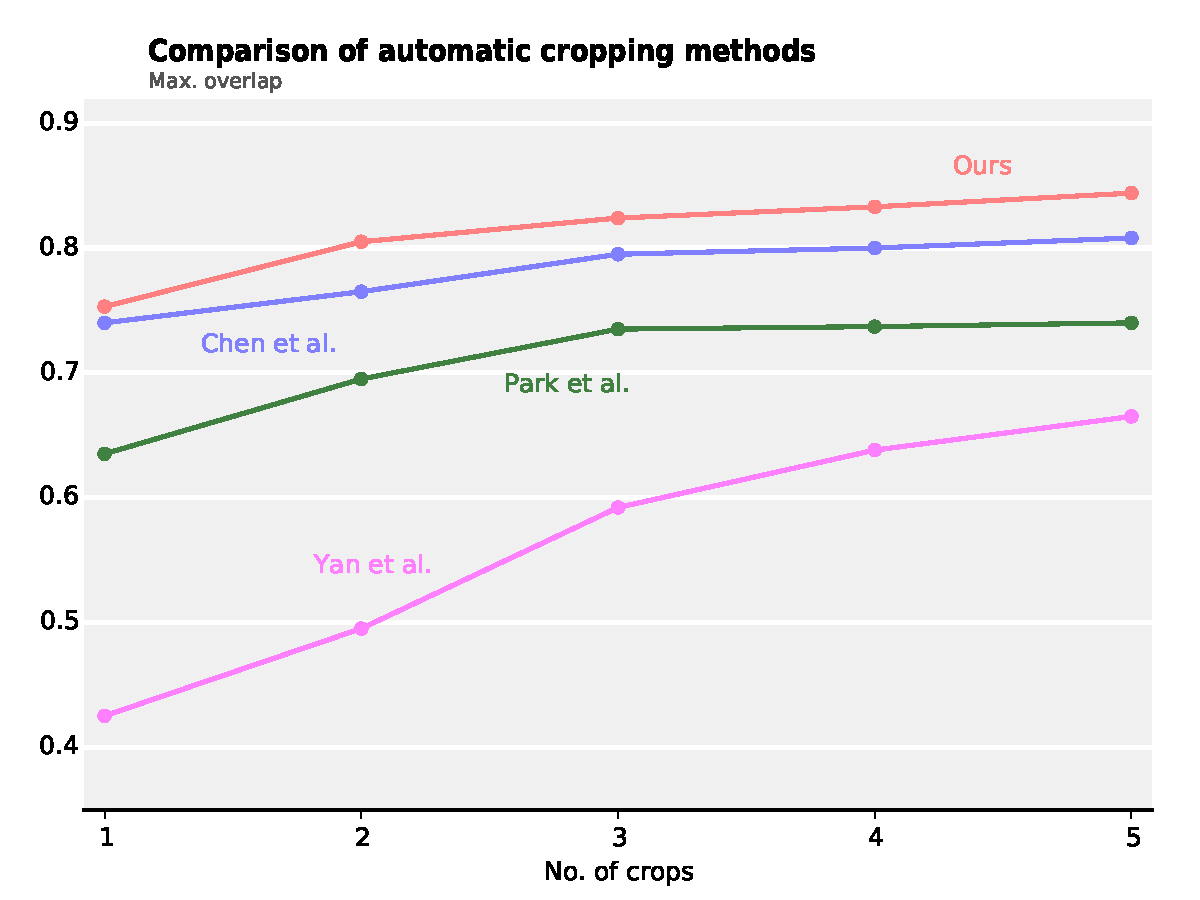
\includegraphics[width=\columnwidth]{../figures/comparison.pdf}
\caption{Quantitative evaluation of various automatic cropping algorithms
	\cite{fang2014automatic,park2012modeling,yan2013learning}.\label{fig:cropping_comparison}}
\end{figure}


%% ----------------------------------------------------------------------------
% BIWI SA/MA thesis template
%
% Created 09/29/2006 by Andreas Ess
% Extended 13/02/2009 by Jan Lesniak - jlesniak@vision.ee.ethz.ch
%% ----------------------------------------------------------------------------

\chapter{Conclusion}

We were initially faced with the problem of reviewing photos from a mobile phone
photo collection, where the photos are used as wallpapers.
This is a two-fold problem concerning the selection of photos to use as
wallpapers, and centering or cropping the image appropriately such that
important or salient areas are shown in an aesthetically pleasing way on the
phone display.

When determining if an image could be used as a wallpaper, it is propagated
through a deep convolutional neural network trained to identify object
categories.
The neuron activations together with annotations are then used to train a SVM.
In practise this works quite well though with a bias towards distant natural
scenes.
Further work could be done in matching personal tastes.

When trained on the Michael dataset and evaluated on the Wookie dataset, an
error rate of 3.7\% is observed where most images are classified correctly.
It is noted that for each annotator there is usually an improvement in precision
when training on just his/her own annotations.
This is to be expected as personal tastes would be better reflected in the
learning phase.
For the case of low correlation between annotations however, it would be
interesting to combine annotations selectively to yield a more aesthetically
pleasing final set of images.

Automatic cropping was selected for retargeting images to a specific aspect
ratio.
For cropping any given image, three cues are considered.
These are: saliency composition, boundary simplicity, and content preservation.
A SVM is trained with features based on these cues using a dataset sourced using
the Reddit web service.
The resulting model and algorithm works quite well, yielding a median maximum
overlap of 0.782 for top 1 crops.
This is an improvement over previous implementations.

Much more could be done to improve the suggested algorithms.

For instance, the datasets used in the selection stage could be improved with a
greater variety of photos as well as a larger number of both photos and
annotations.
Annotators could be asked to annotate based on several keywords or themes,
allowing for a classifier which attempts to adhere to user tastes.
More features could be added during the learning stage.
For instance, the colour distribution or blurriness of the image may change how
suitable an annotator finds the image.

The cropping algorithm shows issues especially in the case where the saliency
map or gradient map does not work as expected.
Future work on enhancing algorithms for generating the two maps should improve
the cropping algorithm.
Further on, image segmentation using SLIC superpixels for example could allow
for more advanced ways in respecting boundary simplicity as well as generating
better crop boundaries in general.




%% ----------------------------------------------------------------------------
% If Appendix is needed
%% ----------------------------------------------------------------------------
\appendix
%% ----------------------------------------------------------------------------
% BIWI SA/MA thesis template
%
% Created 09/29/2006 by Andreas Ess
% Extended 13/02/2009 by Jan Lesniak - jlesniak@vision.ee.ethz.ch
%% ----------------------------------------------------------------------------
\chapter{The First Appendix}

In the appendix, list the following material:

\begin{itemize}
 \item Data (evaluation tables, graphs etc.)
 \item Program code
 \item Further material
\end{itemize}


%% ----------------------------------------------------------------------------
% Bibliography is stored in references.bib file, and can often be found
% online on webpages like dblp.uni-trier.de
%
% To include it in your thesis, run
%  pdflatex main
%  bibtex main
%  pdflatex main
%  pdflatex main
%
% This ensures all references are done correctly.
%% ----------------------------------------------------------------------------

\bibliographystyle{unsrt}
\bibliography{references}

\end{document}

